\documentclass{article}
\usepackage{xeCJK}
  \xeCJKsetup{%
    CJKspace=true,% % true이면 띄어쓰기 사용. 중국어, 일어는 필요 없을수도
    % CJKmath=true,%  % true면 math environment 안에서 CJK 글자 사용
    CJKecglue={}%   % Western과 CJK 사이의 공백 지정: {}로 간격을 없앰
  }
% \setmainfont{Noto Serif}
\setCJKmainfont{Baekmuk Gulim}
\setCJKsansfont{Baekmuk Gulim}
\setCJKmonofont{Baekmuk Gulim}

% Language setting
% Replace `english' with e.g. `spanish' to change the document language
\usepackage[english]{babel}
\usepackage{listings}
\usepackage{minted}
% Remove this draft watermark for the final version
% \usepackage{draftwatermark}

% Set page size and margins
% Replace `letterpaper' with `a4paper' for UK/EU standard size
\usepackage[letterpaper,top=2cm,bottom=2cm,left=3cm,right=3cm,marginparwidth=1.75cm]{geometry}

% Useful packages
\usepackage{amsmath}
\usepackage{comment}
\usepackage{graphicx}
\usepackage{IEEEtrantools}
\usepackage[hyphens]{url}
\usepackage[colorlinks=true, allcolors=blue]{hyperref}

\usepackage{setspace} % CJK가 주인 문서에서 줄간격이 너무 좁을 때
  \onehalfspacing
  % \setstretch{1.25} % custom spacing

\title{Aptos 블록체인: 안전성, 확장성, 향상성 있는 웹3 인프라}
\author{}
\date{2022년 8월 12일\\v1.0 (한글 개정본 0)}

\begin{document}
\maketitle

\renewcommand{\abstractname}{초록}
\renewcommand{\figurename}{그림}

\begin{abstract}
블록체인이 새로운 인터넷 인프라로 부상하면서 수만개의 탈중앙 애플리케이션이 배포되어 왔다. 불행히도, 블록체인은 잦은 중단, 높은 비용, 낮은 처리량 제한 및 수 많은 보안 문제들로 인해 사용이 아직 보편화되지 않았다. 블록체인 인프라는 웹3 시대의 대중화를 위해서 신뢰할 수 있고 확장 가능하고, 비용 효율적이며, 널리 사용되는 애플리케이션의 구축을 위해 지속적으로 발전하는 플랫폼인 클라우드 인프라의 길을 따라야 한다.

우리는 이러한 과제를 해결하기 위해 확장성, 안전성, 신뢰성 및 향상성을 핵심 원칙으로 설계된  Aptos 블록체인을 제시한다. 지난 3년간 전 세계 350명 이상의 개발자들이 Aptos 블록체인을 개발했다~\cite{aptos_core_github}. Aptos는 합의, 스마트 컨트랙트 설계, 시스템 보안, 성능 및 탈중앙성 면에서 새롭고 참신한 혁신을 제안한다. 이러한 기술들의 조합은 웹3 대중화를 위한 기본 구성 요소가 될 것이다:\footnote{Legal Disclaimer: This white paper and its contents are not an offer to sell, or the solicitation of an offer to buy, any tokens. We are publishing this white paper solely to receive feedback and comments from the public. Nothing in this document should be read or interpreted as a guarantee or promise of how the Aptos blockchain or its tokens (if any) will develop, be utilized, or accrue value. Aptos only outlines its current plans, which could change at its discretion, and the success of which will depend on many factors outside of its control. Such future statements necessarily involve known and unknown risks, which may cause actual performance and results in future periods to differ materially from what we have described or implied in this white paper. Aptos undertakes no obligation to update its plans. There can be no assurance that any statements in the white paper will prove to be accurate, as actual results and future events could differ materially. Please do not place undue reliance on future statements.}
 
 \begin{itemize}
  \item 먼저, Aptos 블록체인은 빠르고 안전한 트랜잭션 실행을 위해 Move 언어를 자체적으로 통합하고 내부적으로 사용한다~\cite{move_github}. Move Prover는 Move 언어의 정형검증기로써 스마트 컨트랙트의 불변속성 및 행위에 대한 추가적인 안전을 제공한다. 보안에 대한 이러한 집중을 통해 개발자는 악성 개체로부터 소프트웨어를 더 잘 보호할 수 있다.
  \item 둘째, Aptos 데이터 모델은 유연한 키 관리 및 하이브리드 수탁 옵션을 지원한다. 이는 서명 전 트랜잭션 투명성과 함께 실제 라이트 클라이언트 프로토콜과 함께 보다 안전하고 신뢰할 수 있는 사용자 경험을 제공한다. 
  \item 셋째, 높은 처리량과 낮은 지연 시간을 달성하기 위해 Aptos 블록체인은 트랜잭션 처리의 주요 단계에 모듈화된 파이프라인 방식을 사용한다. 구체적으로는 트랜잭션 전파, 블록 메타데이터 정렬, 병렬 트랜잭션 실행, 배치(batch) 스토리지 및 원장 인증 등이 동시에 운영된다. 이 접근 방식은 사용 가능한 모든 물리적 자원을 완벽하게 활용하고, 하드웨어 효율성을 향상시키며, 매우 병렬적인 실행을 가능하게 한다.
  \item 넷째, 데이터에 대한 사전 지식을 읽고 쓰도록 요구함으로써 트랜잭션 원자성을 파괴하는 다른 병렬 실행 엔진과 달리 Aptos 블록체인은 개발자에게 그러한 제한을 두지 않는다. 임의로 복잡한 트랜잭션이 원자성을 효율적으로 지원하여 실제 애플리케이션의 처리량을 높이고 대기 시간을 단축할 수 있으며 개발을 단순화할 수 있다.
  \item 다섯째, Aptos의 모듈형으로 설계된 아키텍처는 클라이언트 유연성을 지원하고 빈번하고 즉각적인 업그레이드를 위해 최적화되었다. 또한 Aptos 블록체인은 내장된 온체인 변경 관리 프로토콜을 제공하여, 혁신적인 새로운 기술을 신속하게 배포하고 새로운 웹3 사용 사례를 지원할 수 있다.
  \item 마지막으로, Aptos 블록체인은 개별 검증인(validator) 성능 이상의 확장을 위한 미래의 이니셔티브를 실험하고 있다. 모듈식 설계 및 병렬 실행 엔진은 검증인의 내부 샤딩을 지원하며 동종 상태 샤딩은 노드 운영자의 복잡성을 가중시키지 않고 수평적 처리량 확장성을 제공한다.
\end{itemize}

\end{abstract}

\section{서론}
\label{sec:introduction}

웹2 버전의 인터넷에서는 사용자 데이터를 직접 제어하는 중앙 집중식 회사(예: 구글, 아마존, 애플, 메타)가 메시징, 소셜 미디어, 금융, 게임, 쇼핑 및 오디오/비디오 스트리밍과 같은 서비스를 제공했다. 이러한 기업들은 특정 사용 사례에 최적화된 주문형 소프트웨어를 사용한 인프라를 개발하고 클라우드 인프라를 활용하여 이러한 애플리케이션을 사용자에게 배포한다. 클라우드 인프라는 전 세계 데이터 센터(예: AWS, Azure 및 Google Cloud) 내에서 운영되는 임대 가상 머신(VM) 및 베어 메탈 하드웨어와 같은 물리적 또는 가상화된 인프라 서비스에 대한 액세스를 제공한다. 그 결과, 수십억 명의 사용자로 확장할 수 있는 웹2 인터넷 서비스를 구축하는 것이 오늘날 보다 쉬운 적이 없게 되었다. 그러나 웹2에서는 사용자들이 중앙화된 기업에 대한 명백한 신뢰가 요구되며, 이것은 사회적으로 우려가 높아지는 사항이다.

이러한 문제를 해결하기 위해 웹3라는 새로운 인터넷 시대가 시작되었다. 웹3 버전 인터넷에서 블록체인은 사용자가 중개자 또는 중앙화된 기업에 대한 신뢰를 요구받지 않고, 서로 안전하고 안정적으로 상호 작용할 수 있도록 하는 탈중앙, 불변 원장을 제공하기 위해 등장했다. 웹2 인터넷 서비스 및 애플리케이션이 클라우드 인프라를 기본구성요소로 생각하고 의존하는 방식과 유사하게, 탈중앙 애플리케이션은 블록체인을 탈중앙된 인프라 계층으로 사용하여 전 세계 수십억 명의 사용자에게 도달할 수 있다.

그러나 오늘날 많은 블록체인이 존재함에도 불구하고, 웹3의 광범위한 채택은 아직 이루어지지 않았다~\cite{a16_state}. 기술이 계속 고도화되는 가운데 기존 블록체인은 신뢰성이 낮고, 이용자에게 높은 거래 수수료를 부과하고, 처리량 한계가 낮으며, 보안 문제로 정기적인 자산 손실을 겪고, 실시간 대응을 지원할 수 없다. 클라우드 인프라가 웹2 서비스를 수십억의 사용자에게 제공하는 것과 비교하면, 블록체인은 아직 웹3 애플리케이션이 같은 일을 할 수 있게 하지 못했다.

\section{Aptos의 비전}
\label{sec:aptos_vision}

Aptos의 비전은 웹3의 메인스트림 채택을 달성하고 탈중앙 애플리케이션 생태계를 강화해 실제 사용자 문제를 해결할 수 있는 블록체인을 제공하는 것이다. 우리의 임무는 유연하고 모듈화된 블록체인 아키텍처를 제공함으로써 블록체인 신뢰성, 안전성 및 성능에서 최첨단 기술 진보를 이루는 것이다. 이 아키텍처는 빈번한 업그레이드, 최신 기술의 빠른 채택 및 새롭게 부흥한 사용 사례에 대한 최고 수준의 지원을 필요로한다.

우리는 이를 사용하는 커뮤니티가 관리하고 운영하는 탈중앙화 되고, 안전하며, 확장 가능한 네트워크를 상상한다. 전 세계적으로 인프라 수요가 증가하면 블록체인의 컴퓨팅 자원은 이러한 요구를 충족시키기 위해 수평 및 수직적으로 확장된다. 새로운 사용 사례와 기술 진보에 따라 네트워크는 사용자를 방해하지 않고 빈번하면서도 자연스럽게 업그레이드되어야 한다. 인프라에 대한 우려는 이면에서 사라져야 한다. 개발자와 사용자는 키 복구, 데이터 모델링, 스마트 컨트랙트 표준, 자원 사용 트레이드오프, 개인 정보 보호 및 결합성을 위한 다양한 옵션에 액세스할 수 있다. 사용자는 자신의 자산이 안전하고 항상 사용 가능하며, 거의 비용을 지불하지 않고 액세스할 수 있다는 것을 알고 있다. 누구나 알지 못하는 전세계 사람들과 안전하고, 쉽고, 불변하게 거래할 수 있다. 블록체인은 클라우드 인프라만큼 보편적일 것이다.

이 비전을 달성하기 위해서는 상당한 기술 발전이 이루어져야 한다. 지난 3년간 Diem 블록체인(Aptos 블록체인의 전신)을 구축, 개발, 진보 및 배포한 경험을 통해 네트워크가 클라이언트를 방해하지 않고 프로토콜을 지속적으로 업그레이드할 수 있다는 것을 입증했다~\cite{diem_blockchain}. Diem 메인넷은 2020년 초에 여러 지갑 제공업체를 포함한 12개 이상의 노드 운영자에게 배포되었다. 다음 해에 우리 팀은 합의 프로토콜과 핵심 프레임워크를 변경하는 두 가지 주요 업그레이드를 발표했다. 두 가지 업그레이드 모두 다운 타임 없이 완료되었다. Aptos 블록체인에서는, Diem 블록체인의 영감을 받아 안전하고 투명하며 빈번한 업그레이드를 핵심 기능으로 통합하는 동시에 기술 스택에 대한 일련의 급진적인 개선을 수행했다. 특히, 우리는 새로운 트랜잭션 처리 방법과 (\ref{sec:pipelining_batching}절에서 설명됨) 탈중앙 및 네트워크 거버넌스에 대한 새로운 접근 방식을 강조한다.

Aptos 블록체인이 지속적으로 개선되고 성장함에 따라 최신 프로토콜과 설계 선택사항이 포함된 이 백서의 업데이트된 버전을 발행할 것이다. 이 문서의 나머지 부분에서는 Aptos 블록 체인의 현재 상태와 향후 계획을 설명한다.

\begin{figure}
\centering
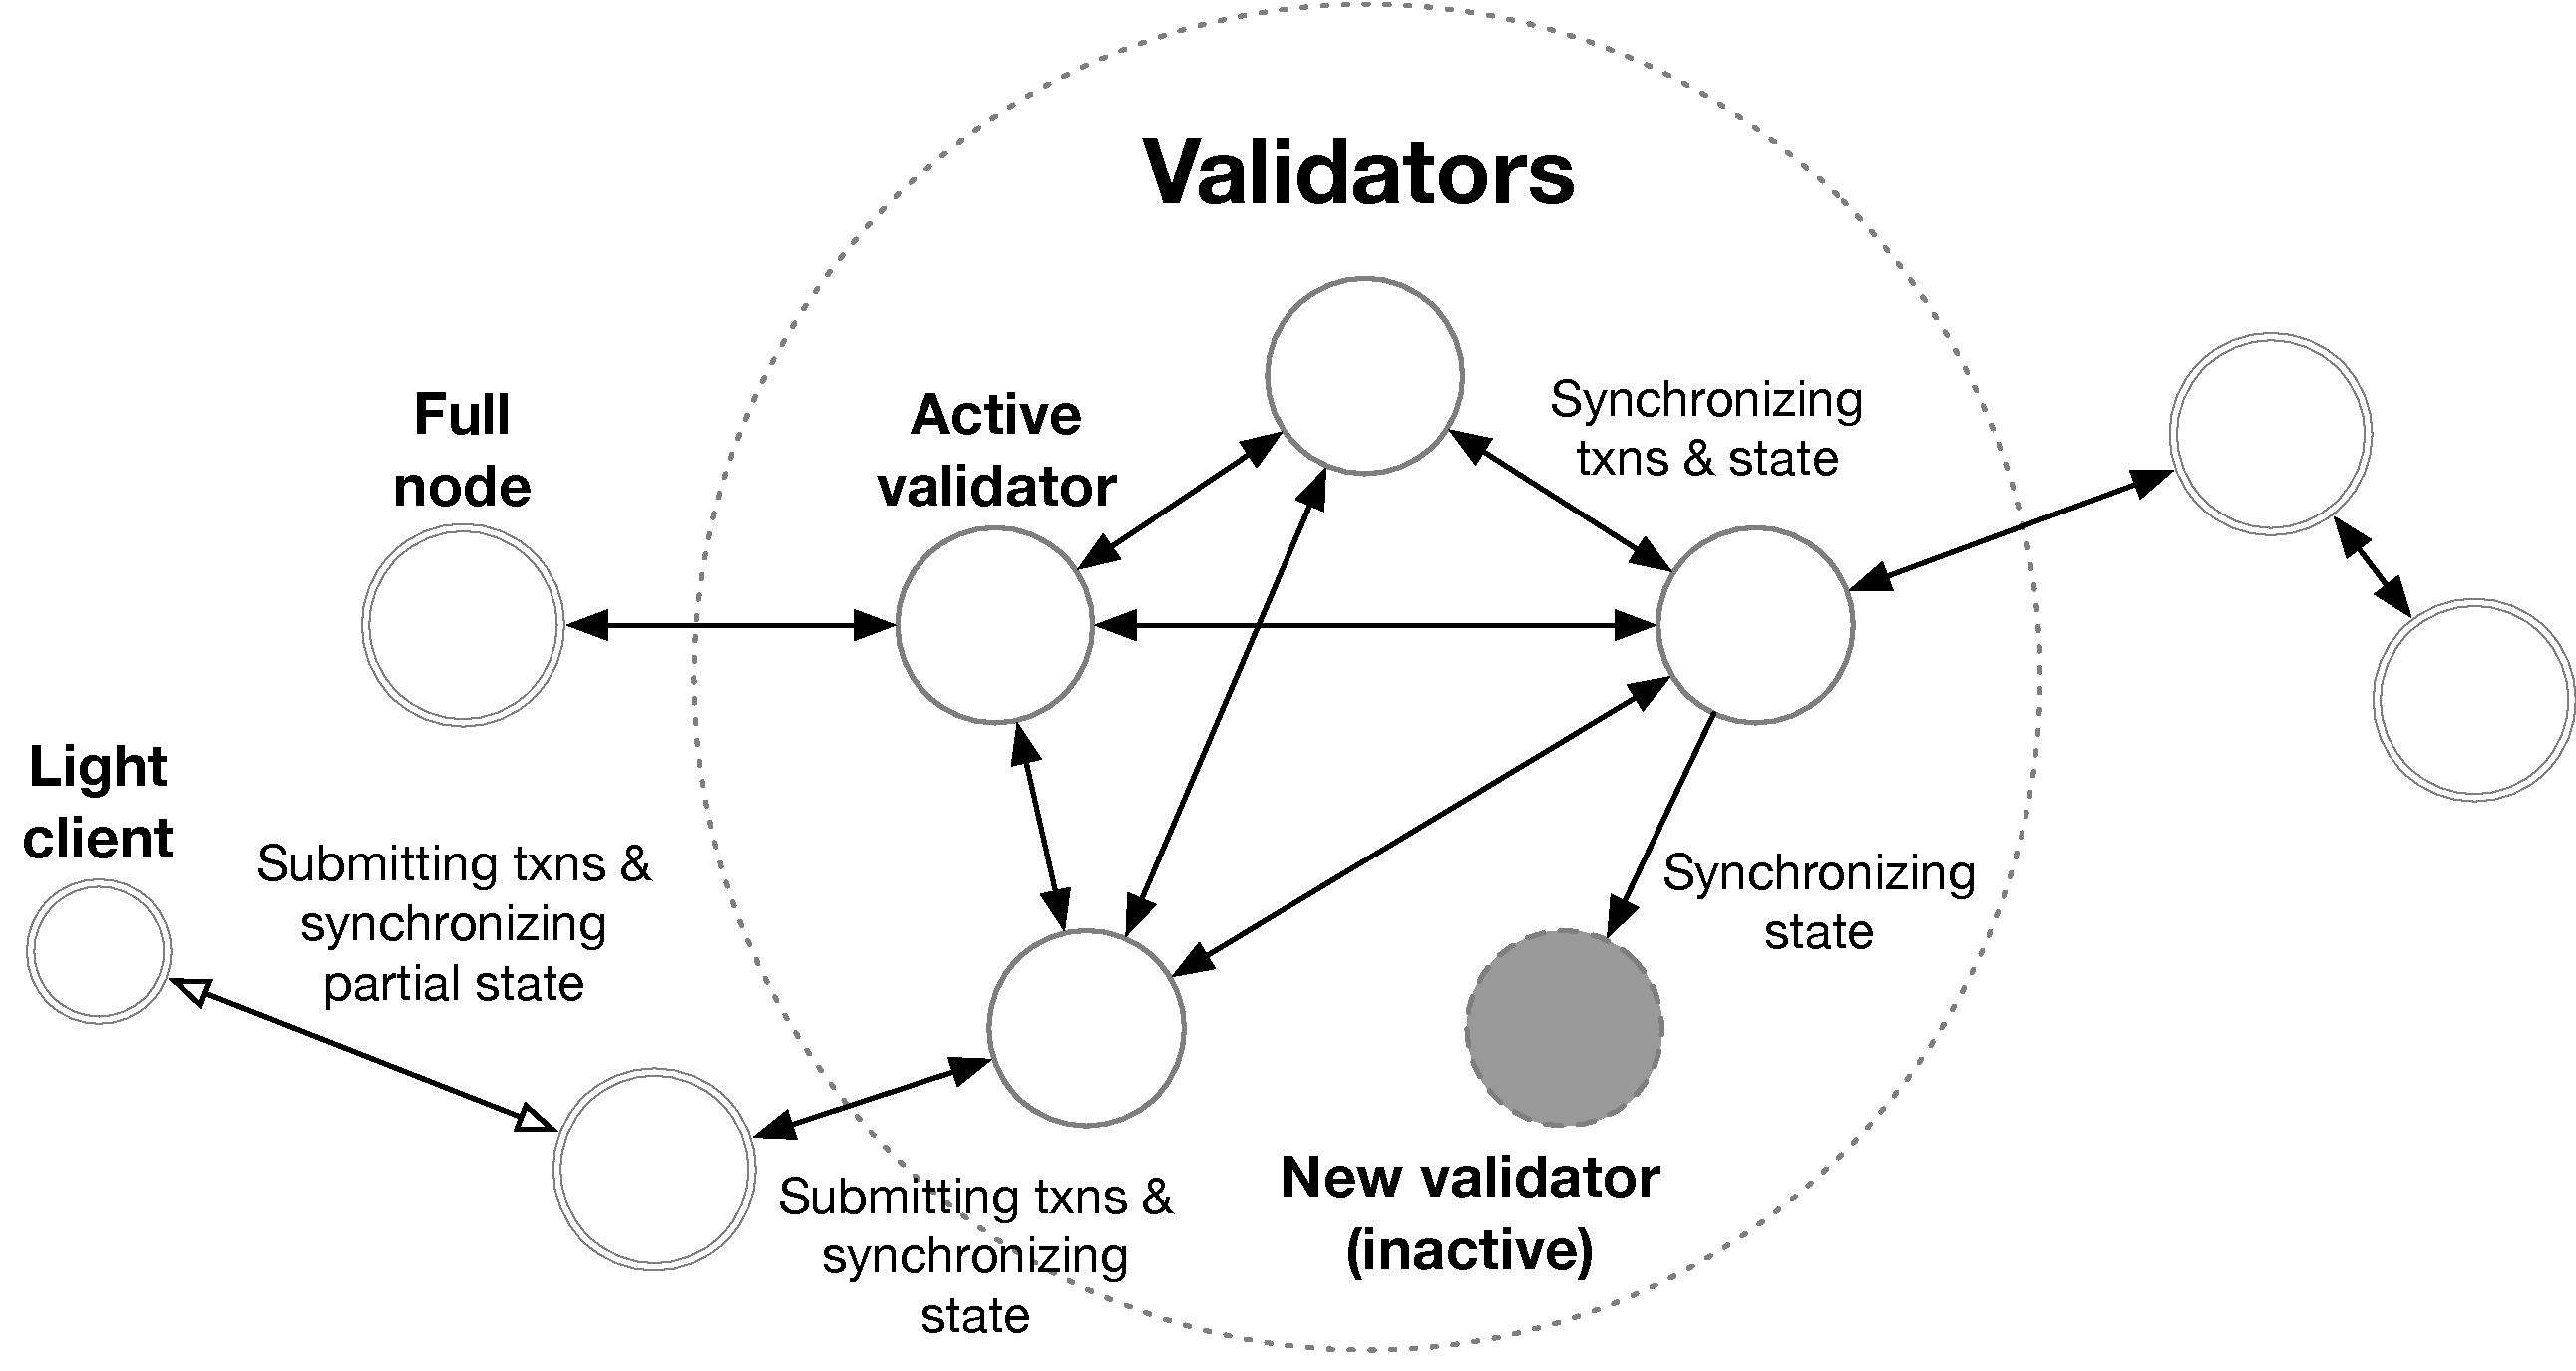
\includegraphics[width=0.9\textwidth]{validators.pdf}
\caption{\label{fig:aptos_ecosystem}Aptos 생태계의 구성 요소.}
\end{figure}

\section{개요}
\label{sec:overview}

그림~\ref{fig:aptos_ecosystem}과 같이 Aptos 블록체인은 비잔틴 장애 허용(BFT)을 사용하여 사용자로부터 트랜잭션을 공동으로 수신하고 처리하는 검증인 집합으로 구성된다. 토큰 소유자는 선택된 검증인에게 토큰을 잠그거나 스테이크 할 수 있다. 각 검증인의 합의 투표 가중치는 스테이킹(staking)된 양에 비례한다. 검증인은 활성되고 합의에 참여할 수 있다. 마찬가지로, 검증인이 참여하기에 충분한 지분을 가지고 있지 않거나, 검증인 집합에서 벗어나 순회하거나, 블록체인 상태를 오프라인으로 동기화 하거나, 과거의 성능이 좋지 않아 합의 프로토콜에 의해 참여하지 않는다고 간주되는 경우에 검증인은 비활성될 수 있다.

클라이언트는 트랜잭션을 제출하거나 블록체인의 상태 및 내역을 조회해야 하는 시스템의 모든 부분에 존재하는 개념이다. 클라이언트는 쿼리된 데이터의 검증인 서명 증명을 다운로드하고 확인할 수 있다. 풀 노드는 검증인 또는 네트워크의 다른 전체 노드에서 트랜잭션 및 블록체인 상태를 복제하는 클라이언트이다. 그들은 저장공간을 회수하기 위해 원하는 대로 트랜잭션 기록 및 블록체인 상태를 제거하도록 선택할 수 있다. 라이트 클라이언트는 현재 검증인 집합만 유지하며 일반적으로 풀 노드에서 부분적으로 블록체인 상태를 안전하게 쿼리할 수 있다. 라이트 클라이언트의 대표적인 예로는 지갑이 있다.

더 많은 채택을 위한 안전하고, 빠르고, 안정적이며, 향상 가능한 웹3 인프라의 요구를 충족하기 위해 Aptos 블록체인은 다음과 같은 핵심 설계 원칙을 기반으로 구축되었다.
\begin{itemize}
    \item 새로운 스마트 컨트랙트 프로그래밍 언어인 Move~\cite{move} 를 통해 간단한 감사 및 기계적 분석으로 빠르고 안전한 실행이 가능함. Move는 Aptos 블록체인의 전신에서 시작되었으며 이 프로젝트의 발전과 함께 계속 개발되고 있음.
    \item 트랜잭션 처리에 대한 배치, 파이프라인 및 병렬화된 접근 방식을 통해 처리량이 매우 높고 대기 시간이 짧음.
    \item 데이터 위치에 대한 사전 지식이 필요한 기존 병렬 실행 엔진과 달리 Block-STM을 통해 임의로 복잡한 트랜잭션으로 원자성을 효율적으로 지원하는 새로운 병렬 트랜잭션 처리.
    \item 빠른 검증인 집단 지분 가중치 로테이션 및 평판 추적을 통해 성능 및 탈중앙화에 최적화.
    \item 새로운 사용 사례와 최신 기술을 수용하기 위한 최고 수준의 설계 원칙인 향상성 및 구성성.
    \item 모듈식 설계를 통해 엄격한 구성요소 수준 테스트와 함께 적절한 위협 모델링 및 원활한 구축을 지원하여 매우 안전하고 안정적인 운영을 보장함.
    \item 프로그래밍과 데이터 모델에 최적화된 1등급 컨셉인 샤딩으로, 탈중앙을 유지하면서 수평적 처리량 확장성을 제공함.
\end{itemize}
\ref{sec:move}절에서는 개발자들이 Aptos 블록체인에서 Move와 어떻게 상호작용하는지 설명한다. \ref{sec:logical}절에서는 논리적 데이터 모델을 설명한다. \ref{sec:user}절에서는 Aptos 블록체인이 어떻게 강력한 검증 방법을 통해 안전한 사용자 경험을 가능하게 하는지 자세히 설명한다. \ref{sec:pipelining_batching}절은 파이프 라인, 배치 및 병렬화에 관한 주요 성능 혁신을 설명한다. \ref{sub:state_sync}절에서는 여러 클라이언트가 다른 노드와 상태를 동기화하기 위한 다양한 옵션이 자세히 나와 있다. \ref{sec:community_ownership}절은 커뮤니티 소유 및 거버넌스에 대한 계획을 설명한다. 마지막으로, \ref{sec:performance}절에서는 탈중앙 유지에 대한 미래의 성능 방향에 대해 논의한다.

\section{Move 개발 언어}
\label{sec:move}

Move는 안전성과 유연성을 특징으로 하는 새로운 스마트 컨트랙트 프로그래밍 언어이다. Aptos 블록체인은 Move의 객체 모델을 사용하여 원장 상태(\ref{sub:ledger_state}절을 참조)를 나타내고, Move 코드(모듈)를 사용하여 상태 전환 규칙을 인코딩한다. 사용자는 새 모듈을 게시하거나, 기존 모듈을 업그레이드하거나, 모듈에 정의된 엔트리 함수를 실행하거나, 모듈의 공용 인터페이스와 직접 상호 작용할 수 있는 스크립트를 포함하는 트랜잭션을 제출한다.

Move 생태계는 컴파일러, 가상 머신 및 기타 많은 개발자 도구를 포함한다. Move는 선형 타입과 같은 개념을 통해 데이터의 소유권을 언어로 명시하는 Rust 프로그래밍 언어에서 영감을 받았다. Move는 리소스에 대한 희소성, 보존 및 접근 제어를 강조한다. Move 모듈은 모든 리소스의 수명, 스토리지 및 액세스 패턴을 정의한다. 이를 통해 코인과 같은 리소스가 적절한 자격 증명 없이 생산되지 않고, 이중으로 사용될 수 없으며, 사라지지 않는다.

Move는 바이트 코드 검증기를 활용하여 신뢰할 수 없는 코드가 있는 경우에도 타입과 메모리 보안을 보장한다. 보다 신뢰할 수 있는 코드를 작성하는 것을 돕기 위해 Move는 정형검증기인 `the Move Prover'~\cite{move_prover} 를 포함하며, 이를 통해 사용자는 Move에 통합된 명세언어를 이용하여 Move 프로그램의 기능적 정확성을 명세하고 확인할 수 있다.

사용자 계정과 해당 계정 내용 외에도 원장 상태에는 Aptos 블록체인의 온체인 구성도 포함되어 있다. 이 네트워크 구성에는 활성 검증인 집합, 스테이킹 속성 및 Aptos 블록체인 내의 다양한 서비스 구성이 포함된다. Move의 모듈 업그레이드 가능성 및 포괄적인 프로그래밍 지원 기능은 원활한 구성 변경을 가능하게 하며 Aptos 블록체인 자체에 대한 업그레이드를 지원한다(두 업그레이드 세트 모두 프라이빗 메인넷에서 다운타임 없이 여러 번 실행되었다).

Aptos 팀은 보다 광범위한 웹3 사용 사례에 대한 지원을 통해 Move를 더욱 강화했다. 첫번째로 Aptos 블록체인은 세분화된 리소스 제어를 가능하게 한다(\ref{sub:ledger_state}절에서 후술). 이는 병렬 실행을 지원할 뿐만 아니라 거의 고정된 비용으로 데이터 액세스 및 변환과 관련된 활동을 수행할 수 있도록 한다. 또한 Aptos 블록체인은 세분화된 스토리지 위에서 테이블 서비스를 구축하여 제공하는데, 이는 단일 계정에서 대규모의 데이터 세트 구축(예: 대규모 NFT 수집)을 가능하게 한다. 마지막으로, Aptos는 완전히 온체인으로 표현되는 공유 혹은 자율 계정을 실현한다. 이를 통해 복잡한 구조 분산형 자율 조직(DAO)이 공동으로 계정을 공유할 수 있을 뿐만 아니라, 이러한 계정을 다양한 리소스를 수집하는 컨테이너처럼 사용할 수 있다.

\section{논리적 데이터 모델}
\label{sec:logical}

Aptos 블록체인의 원장 상태는 모든 계정의 상태를 나타낸다. 원장 상태는 시스템이 실행한 트랜잭션의 수에 대응하는 부호 없는 64비트 정수를 사용하여 버전화된다. 누구나 원장 상태를 수정할 수 있는 트랜잭션을 Aptos 블록체인에 제출할 수 있다. 트랜잭션을 실행하면 트랜잭션 출력 이 생성된다. 트랜잭션 출력에는 원장 상태(쓰기 집합), 결과 이벤트의 벡터(\ref{subsub:events}절을 참조), 가스 소비량 및 실행된 트랜잭션 상태를 조작하기 위한 0개 이상의 작업이 포함된다.

\subsection{트랜잭션}

서명된 트랜잭션에는 다음 정보가 포함된다:
\begin{itemize}
    \item 트랜잭션 인증기(authenticator): 송신인은 하나 이상의 디지털 서명을 포함하는 트랜잭션 인증기를 사용하여 트랜잭션이 인증되었는지 확인한다.
    \item 송신인 주소: 송신인의 계정 주소이다.
    \item 페이로드: 페이로드는 온체인 상의 기존 엔트리 함수를 참조하거나 인라인 바이트 코드(스크립트)로 실행할 함수를 포함한다. 또한 입력 인수 집합은 바이트 배열로 인코딩된다. 피어 투 피어 트랜잭션의 경우, 입력에는 수신자의 정보와 그들에게 전송된 금액의 양에 대한 정보가 포함된다.
    \item 가스비 (지정 통화/가스 단위): 이것은 송신인이 트랜잭션를 실행하기 위해 가스 단위당 지불할 용의가 있는 금액이다. 가스는 연산, 네트워킹 및 저장에 대한 비용을 지불하는 방법이다. 가스 단위는 고유한 실제 값이 없이 이루어진 연산의 추상적인 측정 값이다.
    \item 최대 가스량: 최대 가스량은 트랜잭션이 중단되기 전에 소비할 수 있는 최대 가스 단위이다. 각 계정은 최소 가스비로 가스 가격에 최대 가스량을 곱한 금액을 보유하고 있어야 한다. 그렇지 않으면 트랜잭션 검증 과정 중에 트랜잭션이 폐기된다.
    \item 시퀀스 번호: 트랜잭션의 시퀀스 번호이다. 트랜잭션 시퀀스 번호는 트랜잭션이 실행될 때 송신인의 계정에 저장된 시퀀스 번호와 일치해야 한다. 트랜잭션이 성공적으로 실행되면, 리플레이 공격을 방지하기 위해 계정의 시퀀스 번호가 증가한다.
    \item 만료 시간: 해당 기준 경과 시, 트랜잭션이 더 이상 유효하지 않게 되는 타임스탬프이다.
    \item 체인 id: 트랜잭션이 유효한 블록체인을 식별하여 서명 오류를 방지하는 추가 보호 기능을 제공한다.
\end{itemize}
각 버전 $i$에서 상태 변화는 튜플 $(T_i, O_i, S_i)$로 표현되며, 각각 트랜잭션, 트랜잭션 출력값 및 결과 원장 상태를 포함한다. 결정론적 함수인 $\textsf{Apply}$가 주어졌을 때, 원장 상태 $S_{i-1}$ 를 갖는 트랜잭션  $T_i$ 의 실행은 트랜잭션 출력값인 Oi 와 새로운 원장 상태인 $S_i$를 생성한다. 즉,  $\textsf{Apply}(S_{i-1}, T_i) \rightarrow \langle O_i, S_i\rangle$로 표현할 수 있다.

\subsubsection{이벤트}
\label{subsub:events}

트랜잭션을 실행하는 동안 이벤트를 발생할수 있다. 각 Move 모듈은 자체 이벤트를 정의하고 트랜잭션 실행 시 이러한 이벤트를 발생시킬 시기를 선택할 수 있다. 예를 들어, 코인 전송 중에 송신인과 수신인의 계정은 각각 \mintinline{rust}{SentEvent} 와 \mintinline{rust}{ReceivedEvent}를 발생시킨다. 이 데이터는 원장 내에 저장되며 Aptos 노드를 통해 쿼리할 수 있다. 등록된 각 이벤트에는 고유한 키가 있으며 이 키를 사용하여 이벤트 세부 정보를 쿼리할 수 있다.

동일한 이벤트 키로 발생시킨 여러 이벤트는 이벤트 스트림 즉, 0부터 시작해 순차적으로 증가하는 숫자, 타입 및 데이터를 포함하는 각 엔트리가 포함된 하나의 이벤트 목록을 생성한다. 각 이벤트는 특정 타입에 의해 정의되어야 한다. 특히 제네릭을 사용하는 경우 동일하거나 유사한 타입에 의해 정의된 여러 이벤트가 있을 수 있다. 이벤트는 그와 관련된 데이터를 가진다. Move 모듈 개발자의 경우, 데이터를 변경하고 이벤트를 발생시킨 트랜잭션을 실행하기 전후에 기본 리소스에 대한 변경 사항을 이해하는 데 필요한 모든 데이터를 포함하는 것이 일반 원칙이다.

트랜잭션은 이벤트를 생성할 수만 있으며 이벤트를 읽을 수는 없다. 이 설계를 통해 트랜잭션 실행은 현재 상태와 트랜잭션 입력값의 함수만 될 뿐, 과거 정보(예: 이전에 생성된 이벤트)를 고려하지는 않는다.

\subsection{계정}
\label{sec:accounts}

각 계정은 계정 주소라고 하는 고유한 256비트 값으로 식별된다. 기존 계정에서 전송된 트랜잭션이 \mintinline{rust}{create_account(addr)}라는 Move 함수를 호출하면 원장 상태(\ref{sub:ledger_state}절 참조)에 새 계정이 생성된다. 이러한 경우는 일반적으로 트랜잭션이 아직 생성되지 않은 계정 주소로 Aptos 토큰을 보내려고 시도할 때 발생한다. Aptos는 편의상, 자산 전송 이전에 계정이 존재하지 않을 경우 암묵적으로 계정을 생성하는\mintinline{rust}{transfer(from, to, amount)} 기능도 지원한다.

새 계정을 만들려면, 사용자는 우선 서명 키 쌍  $(vk, sk)$을 생성한다. 다음으로, 주어진 서명 체계에 대한 새 계정 주소는 서명 체계 식별자$(ssid)$와 연결된 공개 검증 키 $vk$ 의 암호화 해시 함수인 $H$ 를 사용하여 도출된다. 즉, $addr = H(vk, ssid)$로 나타낼 수 있다.

주소 $addr$에서 새 계정이 생성된 후, 사용자는 프라이빗 서명 키 $sk$를 사용하여  $addr$에서 보낼 트랜잭션에 서명할 수 있다. 사용자는 $sk$를 변환하여 자체적으로 $sk$를 변경하거나 가능한 위험에 대응할 수도 있다. 이는 계정 주소를 변경시키지는 않는데, 계정 주소는 그 생성 중에 공개 검증 키에서 단 한 번만 파생되기 때문이다.

Aptos 블록체인은 계정을 현실의 정체성과 연동시키지 않는다. 사용자는 여러 개의 키 쌍을 생성하여 복수의 계정을 만들 수 있다. 동일 사용자가 제어하는 계정에는 서로를 잇는 내재된 링크가 없다. 그러나 단일 사용자가 간단한 자산 관리를 위해 하나의 지갑에서 여러 개의 계정을 관리하는 방법이 존재한다. 이러한 유연성은 사용자에게 익명성을 제공하는 동시에 향후에 릴리스(혹은 업데이트) 할 개인정보보호를 위한 기본요소를 실험한다. 단일 사용자 또는 사용자 집합이 소유한 다중 계정도 \ref{subsec:parallel_transaction_execution}절에서 설명한 대로 실행 동시성을 높이기 위한 채널을 제공한다.

\begin{figure}
\centering
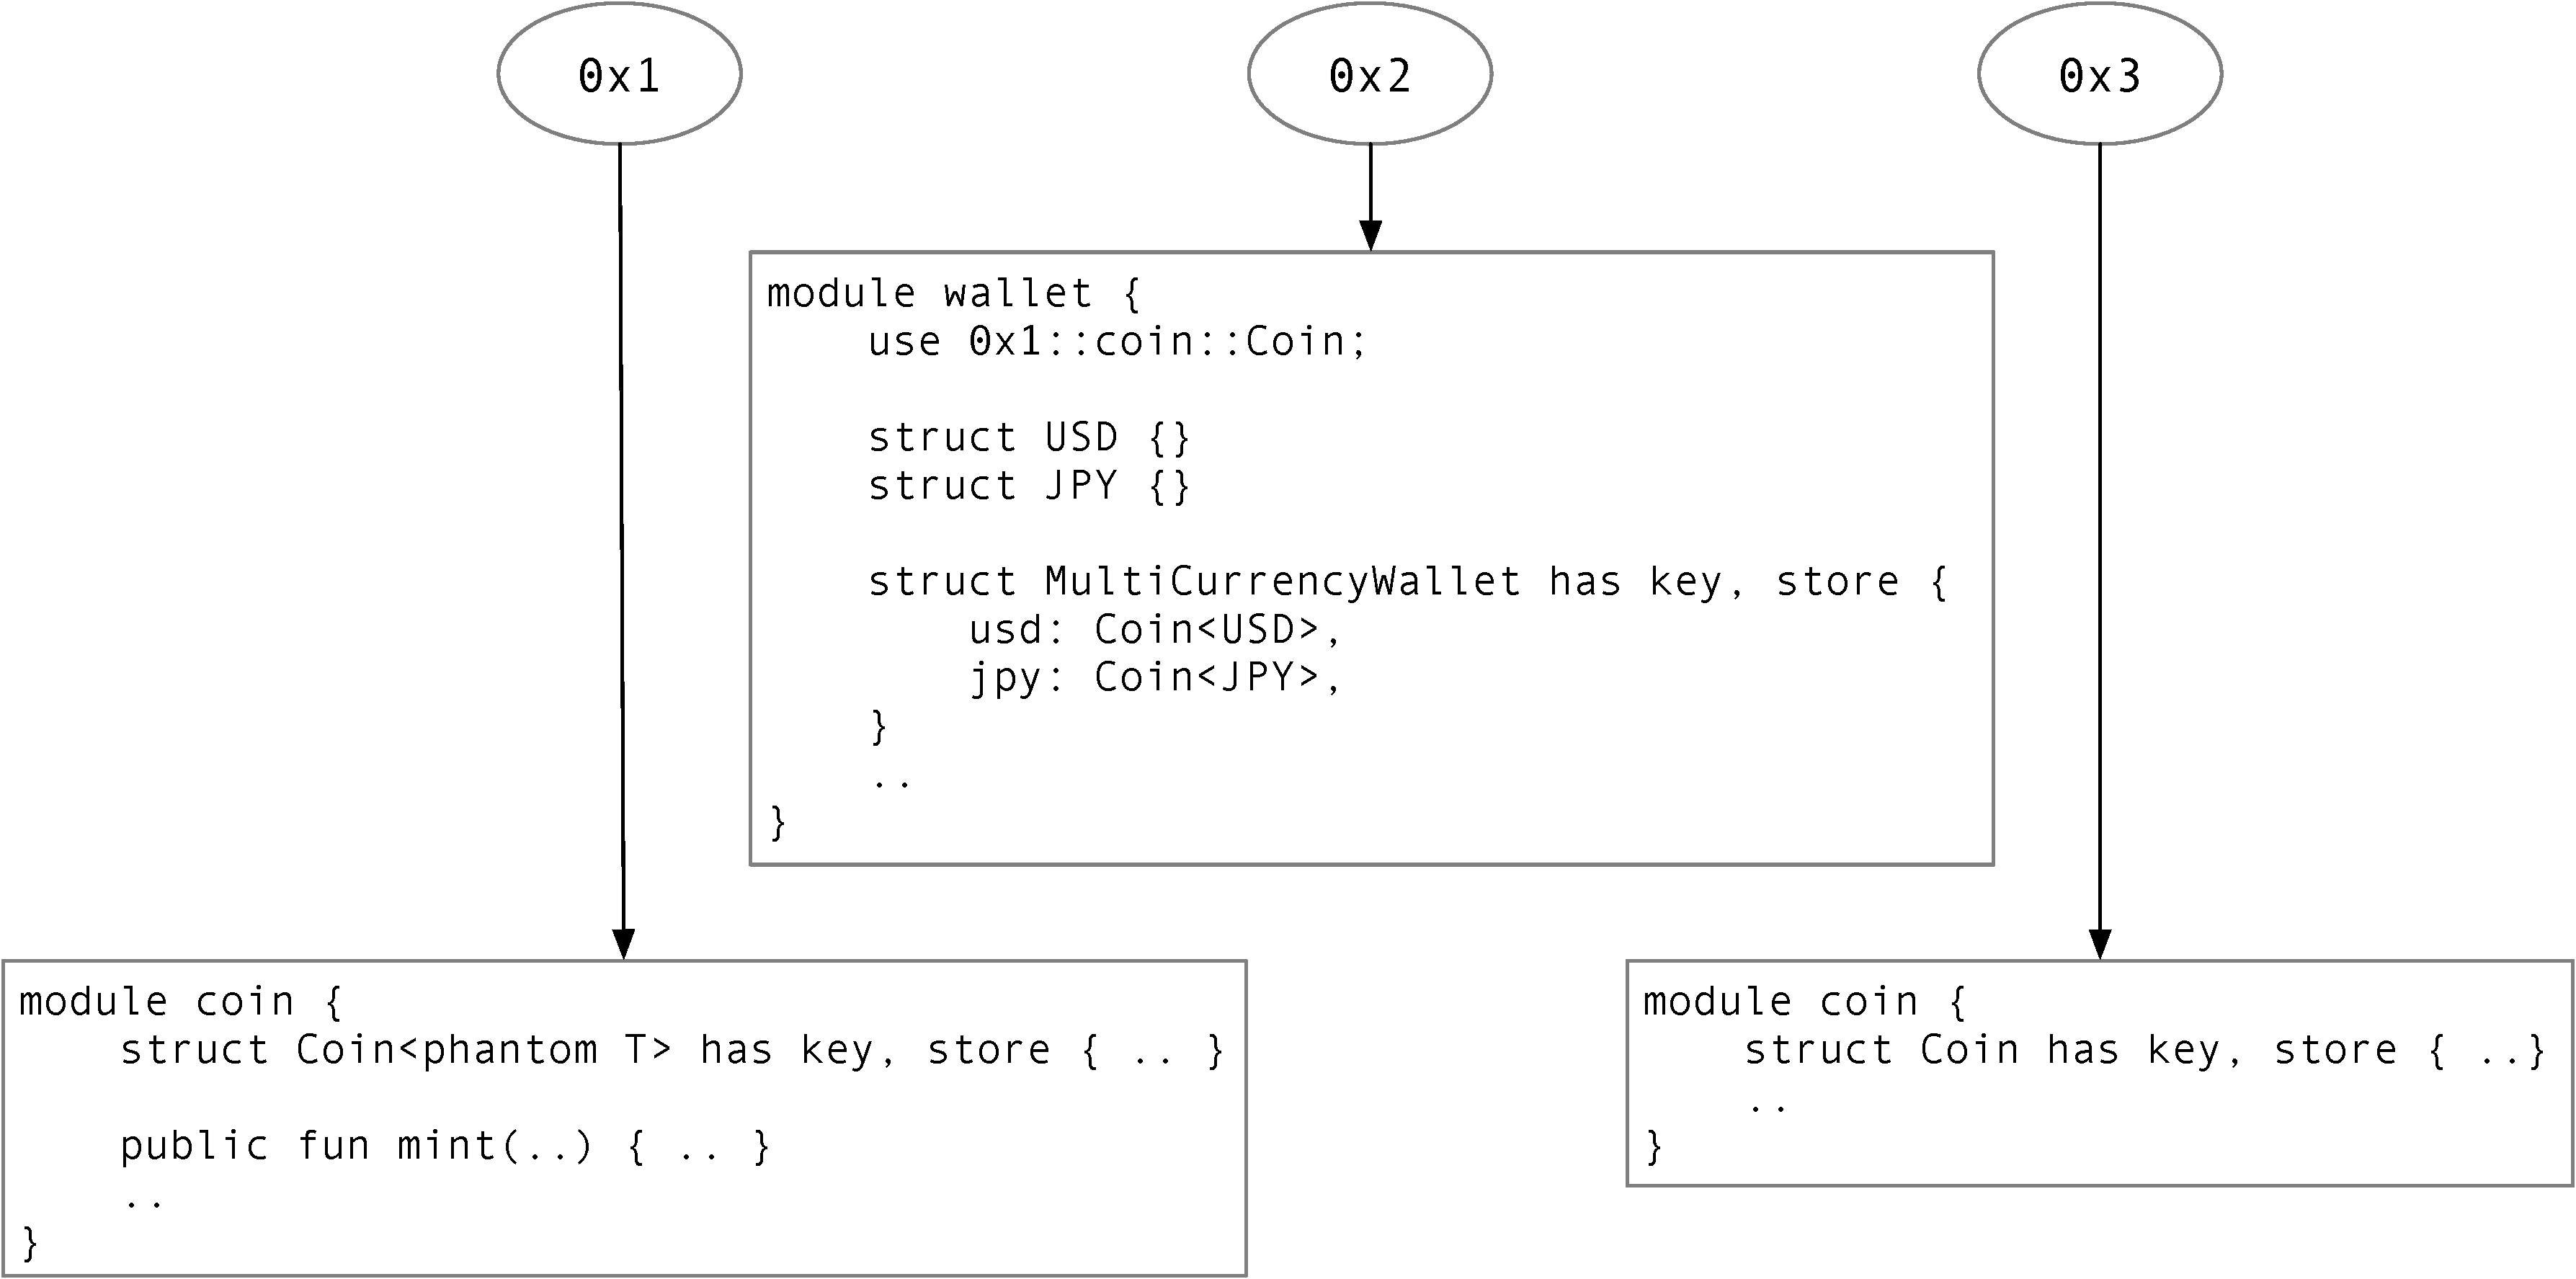
\includegraphics[width=0.85\textwidth]{move_1.pdf}
\caption{\label{fig:move_modules}온체인 Move 모듈의 예시}
\end{figure}

\subsection{Move 모듈}
\label{sec:move_modules}

Move 모듈에는 데이터 타입(구조) 및 절차를 선언하는 Move 바이트 코드가 포함되어 있다. 해당 바이트 코드는 특정 계정 주소로 인식되는데, 해당 계정은 특정 모듈 이름으로 선언된 모듈을 지칭한다. 예를 들어, 그림~\ref{fig:move_modules}의 첫 번째 통화 모듈에 대한 식별자는 \mintinline{rust}{0x1::coin}이다. 한 모듈은 다른 온체인 모듈에 의존할 수 있으며, 그림~\ref{fig:move_modules}에서 지갑 모듈이 보여주듯이 코드 재사용을 가능하게 한다.

각 모듈은 계정 내에서 고유하게 명명되어야 한다. 즉, 각 계정은 주어진 이름으로 최대 하나의 모듈을 선언할 수 있다. 예를 들어, 그림~\ref{fig:move_modules}의 주소 \mintinline{rust}{0x1}에 있는 계정은\mintinline{rust}{coin}이라는 이름의 다른 모듈을 선언할 수 없다. 반면, 주소 \mintinline{rust}{0x3} 의 계정은 \mintinline{rust}{coin} 이라는 이름의 모듈을 선언할 수 있으며 이 모듈의 식별자는  \mintinline{rust}{0x3}이 될 것이다. \mintinline{rust}{0x1::coin::Coin}과 \mintinline{rust}{0x3::coin::Coin}은 서로 다른 타입이며 서로 교환하여 사용하거나 공통 모듈 코드를 공유할 수 없다. 대조적으로  \mintinline{rust}{0x1::coin::Coin<0x2::wallet::USD>}와 \mintinline{rust}{0x1::coin::Coin<0x2::wallet::JPY>}은 동일한 제네릭 타입의 서로 다른 인스턴스화이며, 상호 교환하여 사용할 수는 없지만 공통 모듈 코드를 공유할 수 있다.

모듈은 동일한 주소에 위치한 패키지로 그룹화된다. 이 주소의 소유자는 바이트 코드 및 패키지 메타데이터를 포함한 전체 패키지를 온체인 상에 게시한다. 패키지 메타데이터는 패키지를 업그레이드할 수 있는지 혹은 변경할 수 없는지를 결정한다. 업그레이드 가능한 패키지의 경우 업그레이드가 허용되기 전에 호환성 검사가 수행된다. 즉, 기존 엔트리 포인트 함수를 변경할 필요가 없으며 어떠한 리소스도 메모리에 저장할 수 없다. 그러나 새로운 함수와 새로운 리소스는 추가할 수 있다.

Aptos 블록체인 구축을 위한 핵심 라이브러리와 구성 요소를 내용으로 하는 Aptos 프레임워크는 업그레이드 가능한 일반 모듈 패키지로 정의된다(\ref{subsec:network_governance}절 참조).

\subsection{리소스} 
\label{subsec:resources}

모듈과 유사하게, 계정 주소에도 데이터 값들이 연결될 수 있다. 각 계정 주소 내에서 데이터 값은 해당 타입에 따라 입력되며, 각 타입 당 최대 하나의 값이 해당 계정에 속하게 된다. 그림 \ref{fig:move_data} 은 이에 대한 예시를 나타낸다. 주소 \mintinline{rust}{0x50}은 \mintinline{rust}{0x3::coin::Coin} 이라는 정규화된 타입의 단일 값을 보유한다.\mintinline{rust}{0x3} 은 코인 모듈이 저장된 주소이고, \mintinline{rust}{coin} 은 모듈의 이름이며 \mintinline{rust}{Coin} 은 데이터 타입의 이름이다. 일반 타입의 값도 허용되며, 인스턴스화된 방식에 따라 각각 별개의 타입으로 취급된다. 이것은 다른 인스턴스들이 동일한 함수형 코드를 공유하는 것을 내용으로 하는 확장성 달성에 있어서 필수적인 과정이다.

값을 변환, 삭제 및 게시하는 규칙은 데이터 타입을 정의하는 모듈에서 인코딩된다. Move의 안전성과 검증 규칙은 다른 코드 또는 엔티티가 다른 모듈에서 정의된 데이터 타입의 인스턴스를 직접 생성, 수정 또는 삭제하는 것을 방지한다.

각 주소가 각 타입의 최상위 값 하나만을 갖을 수 있도록 허용하는 것은, 처음에는 제한적인것처럼 보일 수 있다. 그러나 프로그래머는 다른 데이터를 포함하는 래퍼(wrapper) 타입을 내부 필드로 정의할 수 있으므로 실제로는 이러한 특징이 전혀 문제가 되지 않는다. 그림~\ref{fig:move_data}의 \mintinline{rust}{Wallet} 구조는 래퍼 타입을 사용하는 방법의 한 예시이다.

모든 데이터 타입을 온체인 상에 저장할 수 있는 것은 아니라는 점도 유의해야 한다. 데이터 인스턴스가 최상위 값으로 적합하려면 데이터 타입에 키(key) 기능이 명시되어 있어야 한다. 마찬가지로 중첩된 값에도 저장(store) 기능이 필요하다. 두 가지 기능을 모두 갖춘 데이터 타입을 리소스라고 부르기도 한다.

\begin{figure}
\centering
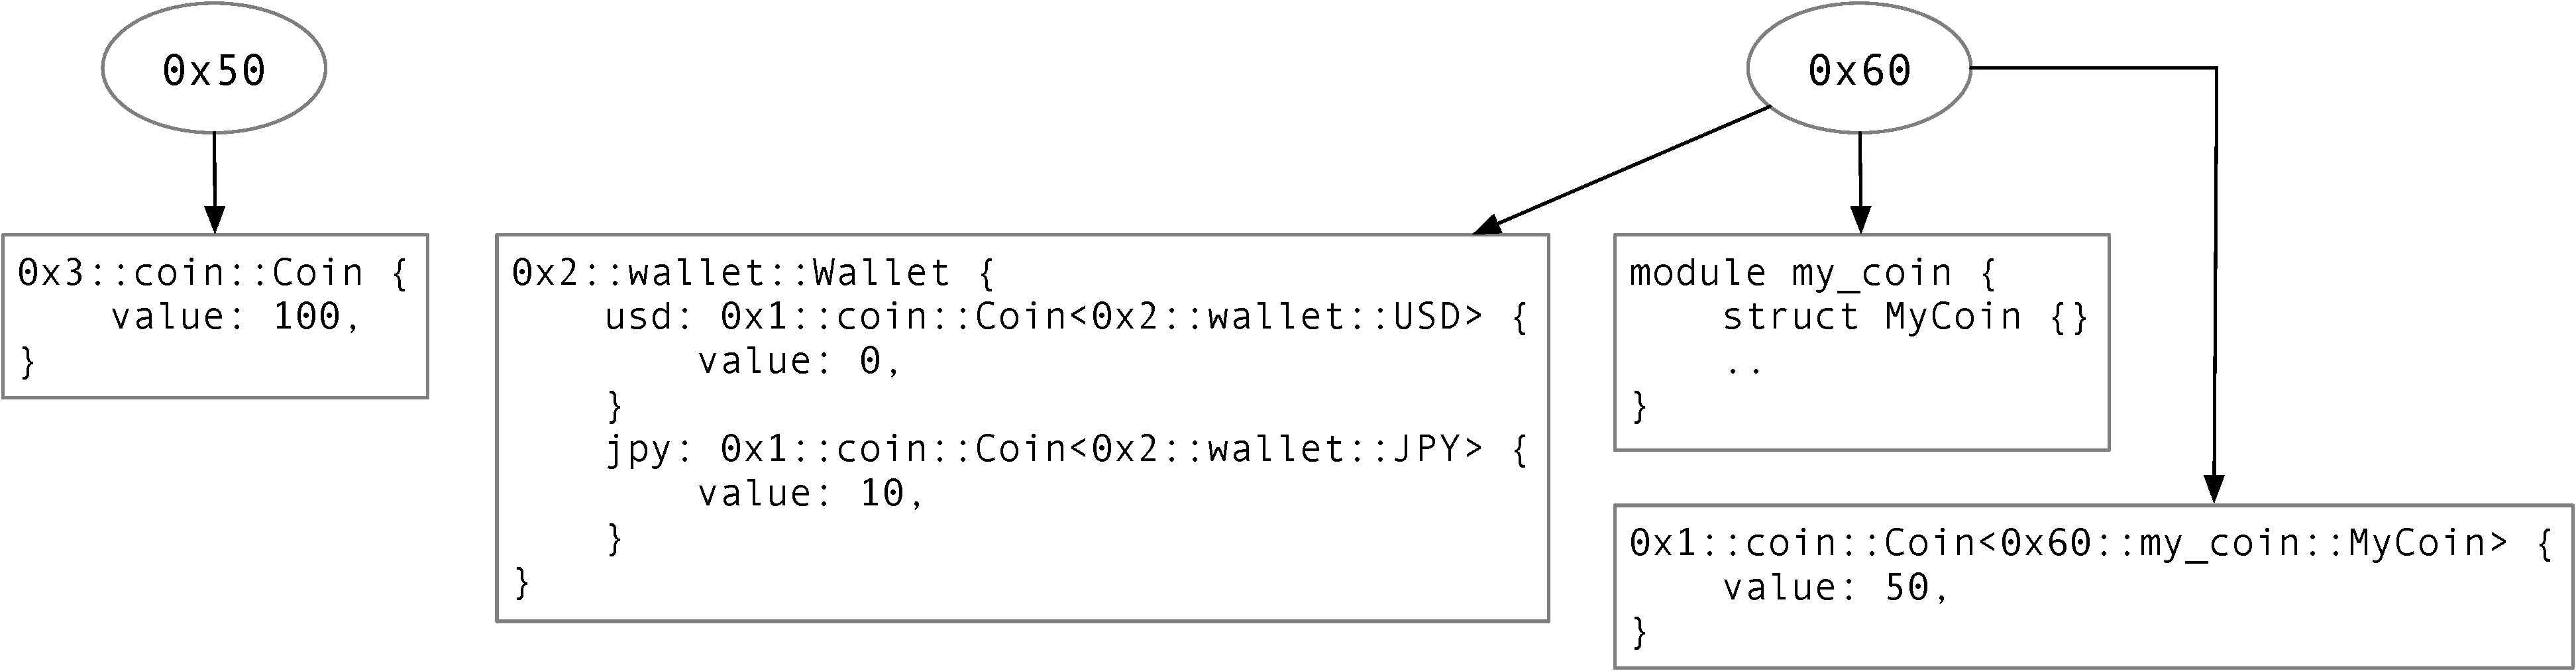
\includegraphics[width=1.0\textwidth]{move_2.pdf}
\caption{\label{fig:move_data}온체인 데이터 예시}
\end{figure}

\subsection{원장 상태}
\label{sub:ledger_state}

Move 가상머신(Move VM) 의 관점에서 각 계정은 일련의 값과 키-값 데이터 구조로 구성된다. 이러한 데이터 구조를 테이블 엔트리(table entries)라고 하며, 이는 Binary Canonical Serialization (BCS) 형태로 저장된다. 이러한 데이터 레이아웃을 통해 개발자는 다수의 계정에 복제된 소량의 데이터와 소수의 계정에 저장된 대량의 데이터 모두를 효율적으로 운영할 수 있는 스마트 컨트랙트를 작성할 수 있다. Move 모듈은 계정 데이터와 유사하지만 독립적인 네임스페이스에 저장된다. 초기 원장 상태는 블록체인 초기화시 초기 계정 집합과 관련 상태를 정의한다.

출시 시 Aptos 블록체인은 단일 원장 상태로 표현된다. 그러나 사용량이 증가하고 기술이 발전함에 따라, Aptos는 처리량을 늘리기 위해 샤드의 숫자를 늘리는 방식으로 확장할 것이며(복수의 원장 상태를 활성화), 샤드를 이용해 자산을 이동시키거나, 자산에 접근하는 트랜잭션을 지원할 것이다. 각 원장 상태는 특정 샤드에 대한 모든 온체인 자산을 유지하고, 스토리지 접근 시에 거의 고정된 비용을 제공하는 세분화된 키 가치 데이터 저장소를 통해 동일한 계정 모델을 제공한다.

\section{안전한 유저 경험}
\label{sec:user}

웹3가 수십억에 달하는 인터넷 사용자들을 끌어들이기 위해서는 안전하고 접근하기 용이한 유저경험을 제공해야 한다. 아래에서 우리는 이러한 목표를 달성할 Aptos 블록체인이 가져올 여러 혁신들에 대해 기술하였다.

\subsection{트랜잭션 실행가능성 보호}
\label{subsec:transaction_replay_protection}

트랜잭션에 서명하는 것은 서명자가 그 트랜잭션이 블록체인에 의해 커밋되고 실행되는 것을 승인한다는 뜻이다. 때때로 사용자는 의도하지 않고 또는 거래가 조작될 수 있는 모든 방법을 완전히 고려하지 않고 거래에 서명할 수 있다. Aptos 블록체인은 이러한 위험을 줄이기 위해 모든 트랜잭션의 실행 가능성을 제한하고 서명자를 무한한 유효성으로부터 보호한다. 현재 Aptos 블록체인은 세 가지 보호 기능을 제공하는데, 전송자의 시퀀스 번호, 트랜잭션 만료 시간 및 지정된 체인 식별자 등이다.
\begin{itemize}
    \item 트랜잭션의 시퀀스 번호는 각 전송자의 계정에 대해 정확히 한 번만 커밋될 수 있다. 결과적으로 전송자는 만약 현재 계정 시퀀스 번호  $\geq$ 트랜잭션 $t$의 시퀀스 번호이면 $t$는 이미 커밋되었거나 영원히 커밋되지 않는다는 것을 확인할 수 있다 ($t$ 에 의해 사용된 시퀀스 번호가 이미 다른 트랜잭션에서 사용되었기 때문).
    \item 블록체인 시간은 \ref{subsubsec:blockchain_time}절에 설명된 대로 높은 정확도와 빈도(보통 1초 미만) 로 진행된다. 만약 블록체인 시간이 트랜잭션 $t$의 만료 시간을 초과하면 마찬가지로 $t$ 는 이미 커밋되었거나 절대 커밋되지 않는다.
    \item 모든 트랜잭션에는 지정된 체인 식별자가 존재하는데, 이는 악의적인 엔티티가 서로 다른 블록체인 환경(예: 테스트넷과 메인넷)간에 트랜잭션을 재생하지 못하도록 한다.
\end{itemize}

\subsection{Move 기반의 키 관리}
\label{sub:move_based_key_management}

\ref{sec:accounts}절에서 논의된 대로, Aptos 계정은 개인 키 손상, 장거리 공격 및 향후 기존의 암호화 알고리즘이 깨질 가능성 관련된 위험을 줄이는 데 도움이 될 수 있는 중요한 기능인 키 로테이션을 지원한다. 또한 새로운 하이브리드 커스터디 모델을 사용할 수 있을 만큼 충분히 유연하다. 이러한 모델 중 하나에서 사용자는 계정의 개인 키를 하나 이상의 관리자와 다른 신뢰할 수 있는 엔티티에게 로테이션시킬 수 있는 능력을 위임할 수 있다. 그리고 이러한 신뢰할 수 있는 엔티티가 특정 상황에서 키를 로테이션시킬 수 있도록 하는 정책을 Move 모듈에 정의할 수 있다. 예를 들어, 엔티티는 많은 신뢰할 수 있는 당사자들이 보유한 $k$-out-of-$n$  다중서명(multi-signature) 키로 표현될 수 있으며 사용자 키 손실을 방지하기 위해 키 복구 서비스를 제공할 수 있다(예: 현재 비트코인의 20\%가 복구 불가능한 계정에 잠겨 있다~\cite{lost_passwords}).

또한 많은 지갑들이 클라우드 인프라에 대한 개인 키 백업, 다자간 컴퓨팅 및 소셜 리커버리와 같은 다양한 키 복구 체계를 지원하지만, 일반적으로 블록체인의 지원없이 구현된다 (즉, 오프체인으로 구현). 결국 각 지갑은 자체 키 관리 인프라를 구현해야 하고 관련 운영은 사용자에게 불투명해진다. 반면 Aptos 블록체인 레이어에서 키 관리 기능을 지원하면 모든 키 관련 작업의 완전한 투명성을 제공할 수 있고 질높은 키 관리를 통해 지갑 구현도 더 간단해진다.

\subsection{사전 서명 트랜잭션 투명성}
\label{sub:pre-signing_transaction_transparency}

오늘날 지갑은 그들이 서명하는 트랜잭션에 대한 투명성을 거의 제공하지 않는다. 결과적으로, 사용자들은 자금을 훔치고 치명적인 결과를 초래할 수 있는 악의적인 트랜잭션에 쉽게 속아서 서명하기도 한다. 이것은 각 트랜잭션에서 액세스하는 모든 온체인 데이터를 열거해야 하는 블록체인의 경우에도 마찬가지다. 그 결과, 현재 사용자를 위한 보호 장치가 거의 없다시피하여 다양한 공격에 취약한 상황이다.

Aptos 생태계는 이를 해결하기 위해 트랜잭션에 서명하기 이전에 사용자에게 트랜잭션 결과를 설명하는 예방 조치인 트랜잭션 사전 실행 서비스를 제공한다. 이를 알려진 이전 공격 및 악의적인 스마트 컨트랙트와 합치면 사기를 줄이는 데 도움이 될 것이다. 또한 Aptos는 지갑이 실행 중인 트랜잭션의 제약을 지시할 수 있도록 한다. 이러한 제약을 위반하면 트랜잭션이 중단되어 악의적인 애플리케이션이나 소셜 엔지니어링 공격으로부터 사용자를 더 안전하게 보호할 수 있다.

\subsection{실용적인 라이트 클라이언트 (light client) 프로토콜}
\label{practical_light_client_protocols}

블록체인 클라이언트와 서버 간 신뢰를 구축하기 위해 API 제공자의 TLS/SSL 인증서에만 의존하는 것은 클라이언트를 충분히 보호하지 못한다. 유효한 인증서가 있더라도 지갑과 클라이언트는 그들에게 제공되는 데이터의 진실성과 무결성에 대한 어떠한 보증도 되지 않는다. 따라서 API 제공업체가 부정확하거나 악의적인 블록체인 데이터를 반환해 제3자를 기만하고 이중 지불 (double-spending) 공격을 할 수 있다.

Aptos는 이를 예방하기 위해 지갑과 클라이언트가 사용할 수 있는 상태 증명 및 라이트 클라이언트 검증 프로토콜을 제공하여 신뢰할 수 없는 제3자 서버가 제공하는 데이터의 유효성을 확인한다. 또한 \ref{subsubsec:period_state_certification}~절의 타임스탬프 기반 상태 증명을 활용함으로써, 라이트 클라이언트는 항상 계정의 최신 상태에 대한 정확한 범위를 확신할 수 있고 (예: 수초 이내), 네트워크 구성의 변경 사항(epoch 변경)만 추적하거나 현재 신뢰할 수 있는 체크포인트(웨이포인트)를 사용하여 최신 상태를 유지하면 된다~\cite{waypoints}. 높은 빈도의 타임스탬프와 낮은 가격의 상태 증명을 결합함으로써, Aptos 블록체인은 클라이언트에게 향상된 보안에 대한 보증을 제공한다.

또한 Aptos 노드는 특정 온체인 데이터 및 계정을 대상으로 하는 증명에 대한 구독을 허용하기 위해 더 세세하게 설정할 수 있는 풍부한 고성능 스토리지 인터페이스도 보유하고 있다. 이를 통해 라이트 클라이언트는 풀 노드를 실행하거나 많은 수의 트랜잭션을 처리 할 필요없이 최소한의 검증 가능한 데이터를 유지할 수 있다.

\section{파이프라인, 배치(batch) 및 병렬 트랜잭션 처리}
\label{sec:pipelining_batching}

Aptos 블록체인의 트랜잭션 처리는 처리량 극대화, 동시성, 엔지니어링 간소화를 위해 여러 단계로 나뉜다. 각 단계는 완전히 독립적이고 개별적으로 작동하여 병렬화가 가능하며 현대적인 슈퍼스칼라(superscalar) 프로세서 아키텍처와 유사하다. 이는 성능 측면에서 상당한 이점을 제공할 뿐만 아니라 Aptos 블록체인에 새로운 방식의 검증인과 클라이언트 간 상호작용을 제공한다. 예를 들어:
\begin{itemize}
\item 특정 트랜잭션이 지속되는 트랜잭션 배치에 포함될 때 해당 클라이언트에게 통보할 수 있다. 지속되는 유효한 트랜잭션은 빠르게 커밋될 가능성이 높다.
\item 지속적인 트랜잭션 배치가 주문되었을 때 클라이언트에게 알릴 수 있다. 따라서 클라이언트는 실행된 트랜잭션 결과 출력의 대기시간을 줄이기 위해 검증인의 원격 실행이 완료되기를 기다리지 않고 로컬 트랜잭션을 실행하도록 선택할 수 있다. 
\item 클라이언트는 검증인이 인증된 트랜잭션 실행을 기다리고 입증된 결과에 대한 상태 동기화를 수행 할 수 있다 (\ref{sub:state_sync}절 참조).
\end{itemize}
Aptos의 모듈러 디자인(modular design)은 단일 모놀리식 아키텍처가 아니라 개별 모듈을 대상으로 하기 때문에 더 빠른 개발 진행과 릴리스 사이클을 지원한다. 마찬가지로, 모듈러 디자인은 단일 시스템을 넘어 검증인을 확장하는 구조화 된 경로를 제공하여 추가적인 컴퓨팅, 네트워크 및 스토리지 자원을 제공한다. 그림~\ref{fig:pipeline} 는 다양한 처리 단계에서 트랜잭션 수명주기를 나타낸다.

\begin{figure}
\centering
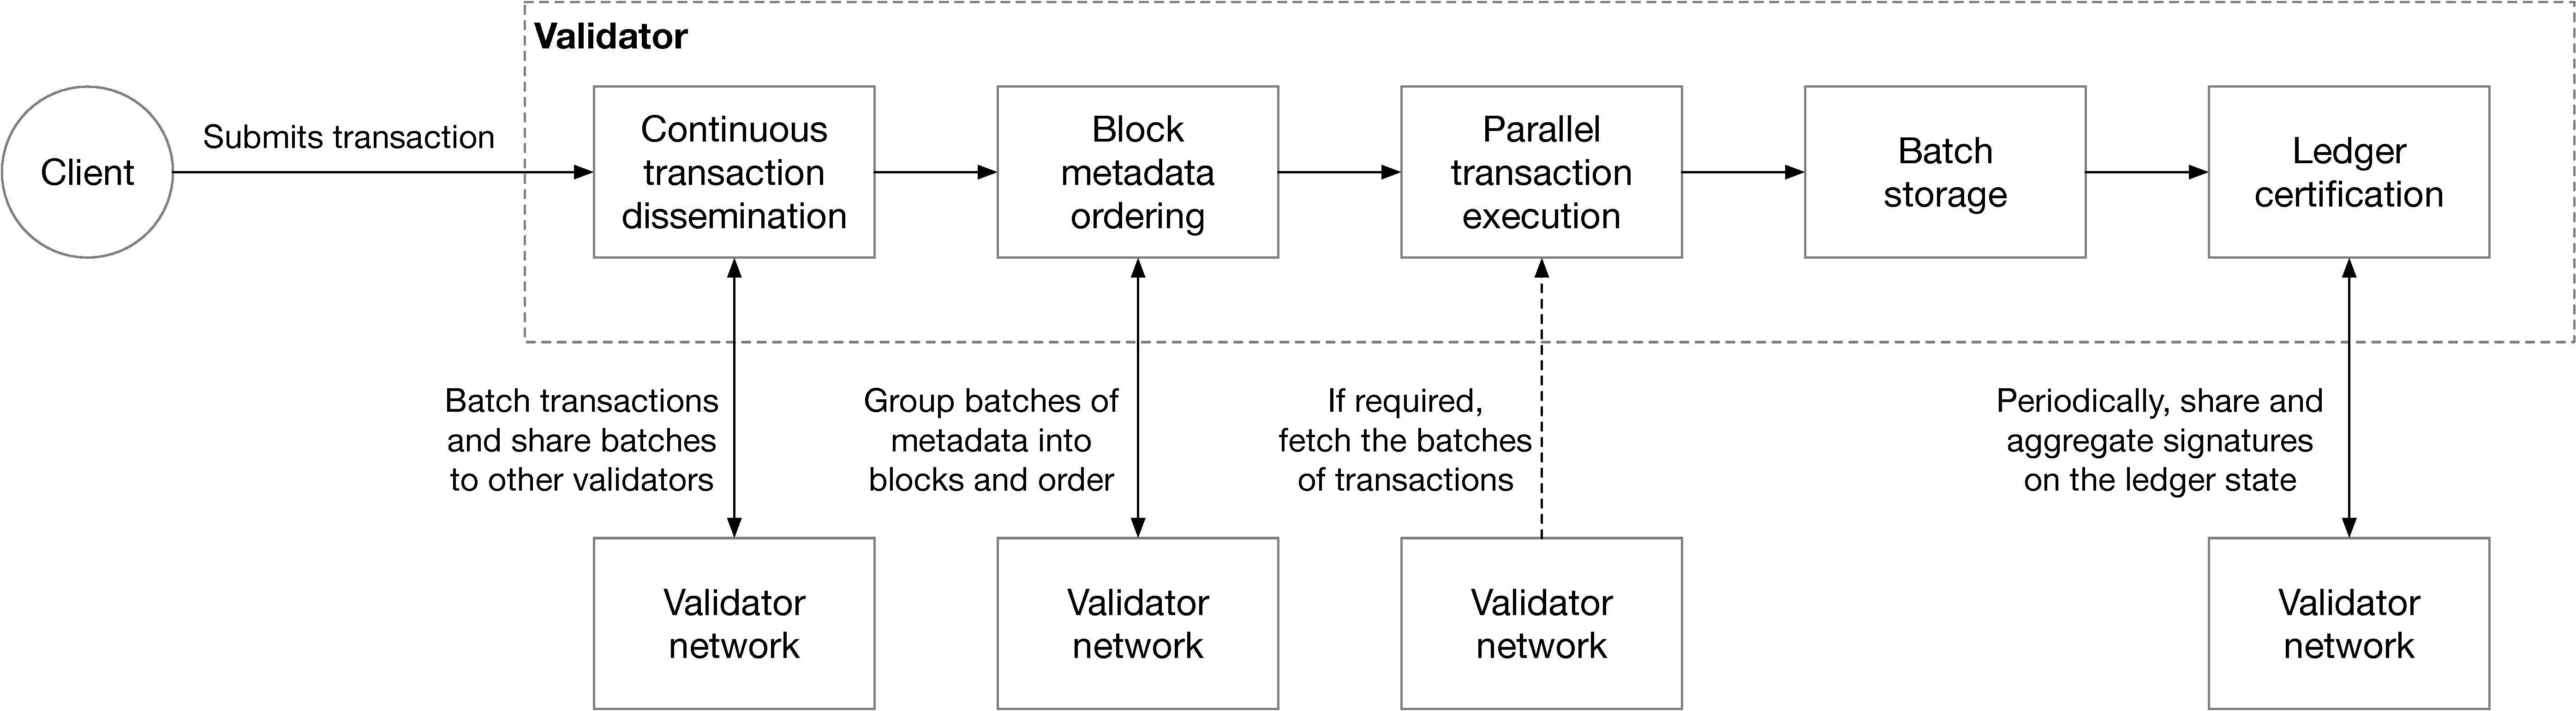
\includegraphics[width=1.0\textwidth]{pipeline.pdf}
\caption{\label{fig:pipeline}트랜잭션 처리 수명 주기. 모든 단계는 완전히 독립적이며 개별적으로 병렬화될 수 있다.}
\end{figure}

\subsection{배치(batch) 프로세싱}
\label{sub:batch_processing}

배치 처리는 Aptos 블록체인에서 효율을 최적화하는 중요한 방법이며 모든 작동 단계에 적용된다. 트랜잭션 배포 중에 트랜잭션들은 각 검증인에 의해 배치로 그룹화되며, 합의 중에 배치는 블록으로 결합된다. 실행, 스토리지 및 원장 인증 단계는 배치로 작동하여 재주문, 중복 계산 또는 서명 검증 등을 고려한 운영 감소, 그리고 병렬 실행을 가능하게 한다.

트랜잭션을 배치로 그룹화할 때 트랜잭션 수집을 위해 배포 전 200 밀리 초 정도 소량의 대기 시간을 발생할 수 있다. 하지만 배치는 최대 대기 시간 및 최대 배치 크기 등 구성성이 용이하여 탈중앙화 네트워크에 맞는 대기 시간과 효율성에 따라 자동으로 최적화 할 수 있다. 또한 배치를 활용하면 효율적인 수수료 시장을 조성하여 트랜잭션의 우선 순위를 정하고 악의적인 클라이언트에 의한 서비스 거부(denial-of-service, DoS) 공격을 피할수 있다.

\subsection{지속적인 트랜잭션 배포}
\label{continuous_txn_dissemination}

Narwhal \& Tusk~\cite{narwhal_tusk}의 주된 내용을 따르며, Aptos 블록체인의 트랜잭션 배포는 합의 과정으로부터 분리된다. 검증인은 사용 가능한 모든 네트워크 리소스를 동시에 활용하여 서로의 트랜잭션 배치를 지속적으로 스트리밍한다. 검증인 $v$에 의해 배포된 각 배치는 지속되며, 배치 다이제스트(digest)의 서명은 $v$로 다시 전송된다. 배치 다이제스트의 $2f+1$ 지분 가중치 서명은 \ref{subsec:block_metadata_ordering}~절에 정의된 합의 요구사항에 따라 가용성 증명(proof of availability, PoAv)을 형성한다. 이러한 증명은 적어도 $f+1$ 지분 만큼의 검증인이 배치를 저장했으며 모든 정직한 검증인이 실행 전에 이를 검색할 수 있다는 것을 보장한다.

무한히 지속적인 트랜잭션 배치는 검증인이 저장 공간 부족으로 인해 고장나게 함으로 서비스 거부 공격을 유발할 수 있다. 이를 방지하기 위해 각 트랜잭션 배치에는 해당 타임스탬프가 있다. 배치의 타임스탬프는 각 검증인의 효율적인 가비지 컬렉션을 가능하게 한다. 또한, Aptos 특유의 검증인 할당 메커니즘은 잠재적인 비잔틴 공격과 같은 가장 극단적인 상황에서도 검증인이 부족하지 않도록 설계되었다. 배치에는 안정적인 저장을 지속하기 위해 계약을 체결하기 전에 검증해야 하는 사이즈 제약 조건이 있다. 마지막으로, 트랜잭션의 중복 제거 및 캐싱을 위한 몇 가지 최적화를 통해 저장 비용을 절감하고 병렬 실행 엔진과의 성능 통합을 보장할 수 있다.

\begin{figure}
\centering
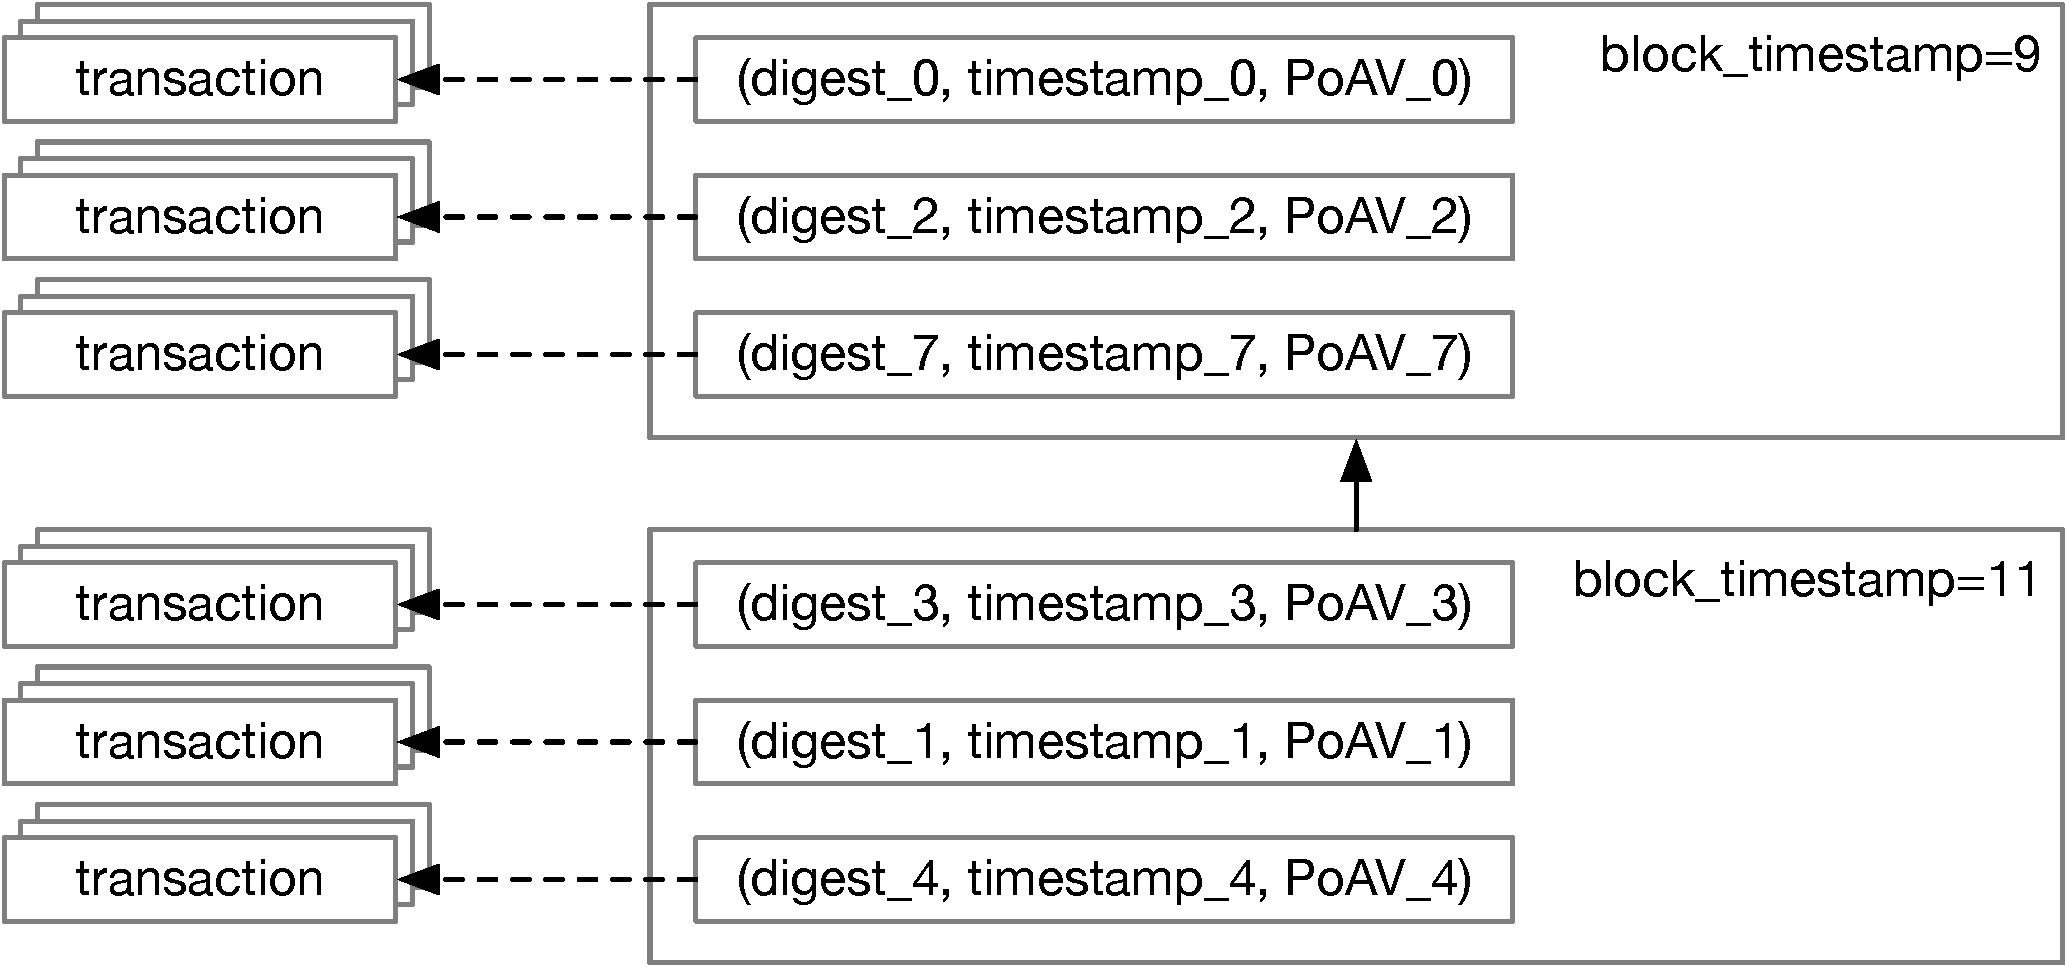
\includegraphics[width=0.8\textwidth]{ordering.pdf}
\caption{\label{fig:block}블록 메타 데이터 정렬은 트랜잭션 배포와 독립적으로 발생}
\end{figure}

\subsection{블록 메타데이터 정렬}
\label{subsec:block_metadata_ordering}

한 가지 일반적인 오해는 합의는 느리고 또한 합의는 블록체인 처리량과 대기 시간 병목의 주요 원인이라는 것이다. Aptos 블록체인의 핵심적인 혁신 중 하나는 트랜잭션 배포, 트랜잭션 실행/저장, 원장 인증 등 합의 단계에서 비합의 관련 작업을 분리하는 것이다. 합의 단계에서 트랜잭션 배포를 분리함으로써 매우 낮은 대역폭(블록 메타데이터 및 증명만)으로 정렬하여, 트랜잭션 처리량을 높이고 대기 시간을 최소화 시킬 수 있다.

오늘날 Aptos 블록체인은 낙관적인 반응형 (optimistically responsive) BFT 합의 프로토콜 중 하나인 DiemBFTv4~\cite{diembft_v4}의 최신 버전을 활용한다. 일반적인 경우 합의는 네트워크 왕복 2회(전 세계적으로 일반적인 왕복 시간은 300밀리초 미만)만 필요하며, 리더 평판 메커니즘을 통해 결함이 있는 검증인들은 동적으로 조정된다~\cite{be_aware}. 온체인 리더 평판 메커니즘은 하나의 윈도우에서 성공적으로 블록을 커밋한 검증인을 승진시키고 참여하지 않은 검증인을 강등시킨다. 이 새로운 메커니즘은 분산 환경의 성능을 크게 향상시키고, 그에 상응하는 적절한 인센티브를 위한 인프라를 제공하며, 실패된 검증인의 처리량과 지연 시간이 네트워크에 미치는 영향을 빠르게 최소화한다.

DiemBFTv4는 부분적인 동기화를 통해 라이브니스를 보장하고 총 검증인의 지분이 $3f +1$ 이상인 비동기를 통해 최대 $f$ 의 지분 가중치 결함 검증인과 함께 안전성을 보장한다. DiemBFTv4는 2019년부터 수십 개의 노드 운영자와 다중 지갑을 지원하는 생태계를 통해 여러 번 테스트 되었다. 우리는 또한 우리의 최근 연구(예: \cite{bullshark})에 대한 실험과, 블록 히스토리 및 관련 통신에 의존하는 기타 프로토콜로 블록 메타 데이터 정렬과 최종성을 결정하는 실험을 하고 있다.

합의 블록과 프로포절의 타임스탬프는 리더에 의해 제안되고 그림~\ref{fig:block} 같이 다른 검증인에 의해 합의된다. 각 합의 블록에는 배치 메타데이터와 증명만 포함된다. PoAv는 주문 후 실행 단계에서 트랜잭션 배치를 사용할 수 있도록 하기 때문에 블록에서 실제 트랜잭션이 필요하지 않다 (\ref{continuous_txn_dissemination}절). 검증인은 증명 및 블록 메타데이터 기준이 충족되는지 확인한 후 리더의 제안에 투표할 수 있다(예: 프로포절 타임스탬프 $\leq$ 블록 만료 시간).

\subsubsection{블록체인 시간}
\label{subsubsec:blockchain_time}

Aptos 블록체인은 제안된 모든 블록에 대해 합의된 대략적인 물리적인 타임스탬프를 채택하고, 그에 상응하여 해당 블록 내의 모든 트랜잭션을 채택한다. 이 타임스탬프는 많은 중요한 사용 사례를 가능하게 한다. 예를 들어:

\begin{itemize}
\item 스마트 컨트랙트내에 시간에 의존적인 로직. 예를 들어, 한 개발자는 경매의 모든 입찰이 목요일 정오 전에 접수되어야 한다고 인코딩하고 싶어한다.

\item 오라클이 온체인 데이터를 게시함에 따라 실제 세계의 데이터로부터 연관된 이벤트와 지연을 처리하려면 정확하고 신뢰할 수 있는 온체인 타임스탬프가 필요하다.

\item 클라이언트는 블록체인과 관련하여 자신이 얼마나 최신 상태인지 식별할 수 있다. 보안상의 이유로, 불필요한 데이터와 장기간의 공격을 피하기 위해 계정 상태가 업데이트되었을 때 클라이언트가 정확한 타임스탬프에 액세스할 수 있어야 한다.

\item 신뢰할 수 있는 타임스탬프로 블록체인을 감사하면 법적으로 시행되는 지불금이 예상 요구 사항을 충족하는지 확인하는 것과 같은 오프체인 이벤트와 강한 연관성을 제공할 수 있다.

\item 트랜잭션 만료는 가장 최근에 커밋된 타임스탬프를 기반으로 한다. 클라이언트 트랜잭션에 대한 추가적인 보호 수단으로써 클라이언트는 \ref{subsec:transaction_replay_protection}절에 설명된 대로 트랜잭션 만료 시간을 선택할 수 있다.
\end{itemize}

Aptos 블록체인은 블록 내의 모든 트랜잭션에 대한 타임스탬프와 관련하여 다음과 같은 내용을 보장한다.

\begin{itemize}
\item 시간은 블록체인에서 선형적으로 증가한다. 즉, 만약 블록 B1 < 블록 B2 인 경우, B1.시간 < B2.시간이다.

\item 트랜잭션 블록이 타임스탬프 $T$와 합의된 경우, 최소 $f + 1$개의 정직한 검증인이 이전의 $T$ 로 결정되었다. 정직한 검증인은 자체 클럭 $\geq$ 타임스탬프 $T$ 인 경우일 때만 블록에 투표한다. \ref{continuous_txn_dissemination}절을 참조.

\item 트랜잭션 블록에 타임스탬프 $T$와 합의된 서명 쿼럼(quorum)이 있는 경우, 정직한 검증인은 자신의 클럭 $\geq$ 타임스탬프 $T$가 될 때까지 다른 검증인에게 이와 같은 블록을 제공하지 않는다.
\end{itemize}

가장 최근의 타임스탬프는 모든 커밋된 블록에서 업데이트 되며 해당 블록의 모든 트랜잭션의 타임스탬프로 사용된다. 네트워크가 동기화 되면, 트랜잭션 블록은 네트워크를 왕복할때 마다 커밋되며 빠른 업데이트와 매우 안정적인 클럭을 제공한다. 원하는 경우 트랜잭션 블록 내에서 세분화된 순서를 결정할 수 있다.

\subsection{병렬 트랜잭션 실행}
\label{subsec:parallel_transaction_execution}

합의 블록 메타데이터가 주문되면 모든 검증인, 전체 노드 또는 클라이언트가 트랜잭션을 실행할 수 있다. 최소 $2f + 1$ 지분 가중치의 검증인은 제안된 배치에 대한 트랜잭션을 유지한다. 트랜잭션 배포는 지속적이기 때문에 추가적인 검증인은 시간이 지남에 따라 트랜잭션 배치(batch)를 받는다. 정직한 검증인이 실행 단계에 도달할 때까지 주문된 배치에 대한 트랜잭션을 받지 못한 경우 이를 $2f + 1$ 지분 가중치의 검증인으로부터 다운로드 할 수 있으며, 적어도 $f + 1$ 지분 가중치의 검증인은(스테이크 가중 PoAv 서명자의 절반) 정직하다고 판단할 수 있다.

모든 블록체인의 중요한 목표는 가능한 많은 병렬 실행을 가능하게 하는 것이다. Aptos 블록체인은 데이터 모델과 실행 엔진 모두를 이러한 방향으로 발전시킨다.

\subsubsection{병렬 데이터 모델}

Move 데이터 모델은 기본적으로 데이터 및 모듈의 글로벌 주소지정(addressing)을 지원한다. 데이터와 계정에서 충돌이 없는 트랜잭션들은 병렬로 실행할 수 있다. Aptos 블록체인에서 사용하는 파이프라인 디자인을 고려할 때 트랜잭션 그룹을 재정렬하면 충돌 횟수가 줄어들어 동시성이 향상된다.

트랜잭션이 동일한 체인 값 세트를 수정하더라도, 트랜잭션 실행 과정의 대부분이 병렬화 될 수 있다. Aptos 블록체인은 \emph{delta-write}라는 새로운 개념을 소개하는데, 이것은 계정의 변화된 상태를 기술하는 것이 아니라 변화 자체를 기술한다(정수의 덧셈 예로써, 더해진 최종 값이 아니라 더할 값). 모든 트랜잭션은 병렬로 처리될 수 있으며, 결정론적 결과를 보장하기 위해 delta-write는 충돌 값에 올바른 순서로 적용된다.

Aptos 블록체인은 동시성(예 : 읽기/쓰기 힌트를 활용)과 인간공학을 향상시키는 방식으로 데이터 모델을 계속 지속적으로 개선시켜 개발자가 온체인 값을 더 자연스럽게 생성, 수정 및 구성할 수 있도록 한다. Move는 이러한 개선들이 언어 차원에서와 플랫폼 특정 기능을 통해 가능하도록 유연성을 제공한다.


\begin{figure}
\centering
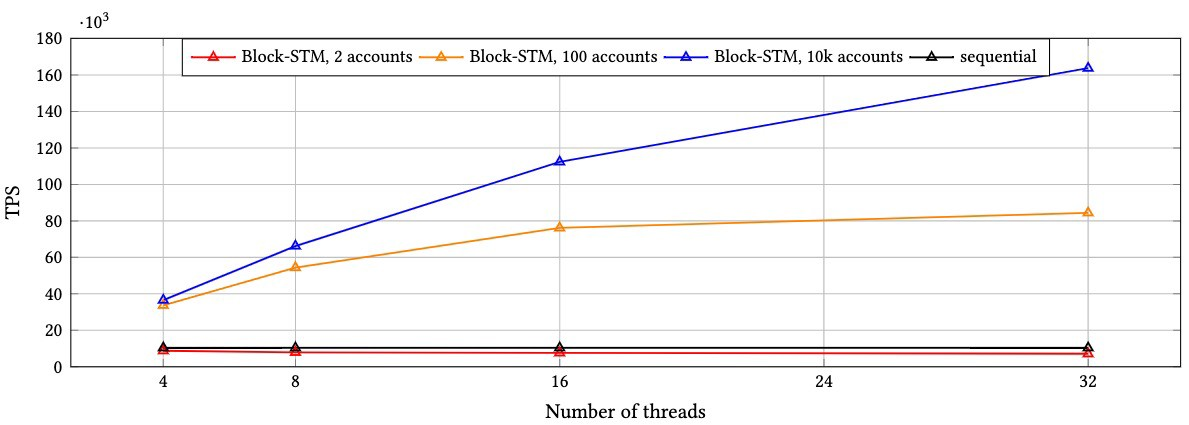
\includegraphics[width=0.95\textwidth]{perf.jpg}
\caption{\label{fig:perf}Block-STM에 (컴포넌트만 해당) 대해 각기 다른 물리적인 코어 개수와 경합으로 퍼포먼스 테스트를 진행}
\end{figure}

\subsubsection{병렬 실행 엔진}

Block-STM 병렬 실행 엔진은 특정 순서에 따라 최적의 병렬화를 위해 낙관적 동시성 제어와 함께 주문한 트랜잭션 세트의 충돌을 감지하고 관리한다~\cite{block_stm}.

트랜잭션 배치는 병렬로 실행되고 실행 후 검증된다. 실패한 검증은 재실행으로 이어진다. Block-STM은 write-write 충돌을 피하기 위해 다중 버전의 데이터 구조를 사용한다. 동일한 위치에 대한 모든 쓰기는 트랜잭션 ID와 트랜잭션이 낙관적으로 다시 실행된 횟수를 포함하는 버전과 함께 저장된다. 트랜잭션 $tx$ 가 메모리 위치를 읽으면 다중 버전 데이터 구조에서 사전에 설정된 순서에 맞게 $tx$ 이전에 가장 높은 트랜잭션이 해당 위치에 기록된 값을 불러온다.

Block-STM은 이미 Aptos 블록체인에 통합되어 있다. Block-STM 성능의 잠재력을 이해하기 위해 메모리 내 데이터베이스가 있는 분리된 실행 전용(엔드 투 엔드가 아닌) 벤치마크로서 P2P Move 트랜잭션(트랜잭션 당 8개의 읽기 및 5개의 쓰기)에 대한 실험을 진행했다. Block-STM 실행 결과는 그림 \ref{fig:perf}과 같다. 모든 블록에는 10,000개의 트랜잭션이 포함되어 있으며 계정 수가 충돌 수준과 경합 수준을 결정한다.

낮은 경합 수준에서 Block-STM은 32개의 스레드로 순차적 실행에 비해 16배 속도를 달성하는 반면, 높은 경합수준에서 Block-STM은 8배 정도의 속도를 달성한다. 블록체인 공간의 다른 병렬 실행 엔진과 차별화된 Block-STM은 사용자의 힌트없이 모든 워크로드에서 동적이고 투명하게 고유한 병렬 처리를 진행한다. BlockSTM은 읽거나 데이터 위치에 대한 선행 지식이 필요한 병렬 실행 환경과 비교하여 보다 복잡한 트랜잭션을 동시에 지원할 수 있다. 이러한 속성은 트랜잭션을 더 효율적이게 하고 트랜잭션의 수와 비용을 줄일 수 있으며 사용자 대기 시간이 낮아진다. 가장 중요한 것은 아토믹 트랜잭션을 여러 작은 트랜잭션으로 분할하면 단일 트랜잭션의 복잡한 상태 결과를 방지할 수 있다. 표현형 트랜잭션 시맨틱을 Block-STM에서 병렬 실행과 페어링하면 개발자가 두 영역의 장점을 모두 활용할 수 있다.

블록 메타데이터 정렬 단계는 병렬 실행 단계에서 트랜잭션 재정렬을 배제하지 않는다는 점에 유의해야 한다. 병렬 실행의 동시성을 최적화하기 위해 하나 이상의 블록에서 트랜잭션을 재정렬 할 수 있다. 여기에서 유일한 요구 사항은 모든 정직한 검증인에게 재정렬이 결정되어야 한다는 것이다. 병렬 실행을 최적화하고 재주문에 무작위 배정을 추가하면 성능이 향상되고 수익성 있는 검증인 트랜잭션 재정렬을 위한 MEV 기술을 방지할 수 있다. ``Order-then-reveal'' MEV 저항 전략 또한 이 파이프라인 디자인에 통합된다.

Block-STM과 트랜잭션 재정렬은 병렬 실행을 높이기 위한 보완적 기술이다. 이는 추가적인 동시성을 위해 트랜잭션 읽기/쓰기 액세스 힌트와 결합 할 수 있다.

\subsection{배치(batch) 스토리지}

병렬 실행 단계는 그룹의 모든 트랜잭션에 대한 쓰기 세트를 형성한다. 이 쓰기 세트은 최대 실행 속도를 위해 메모리에 저장한 후 다음 블록 또는 실행할 블록 세트의 캐시로 사용될 수 있다. 덮어쓰기는 안정적인 스토리지에 한 번만 기록하면 된다. 메모리 내 쓰기 세트를 저장하기 전에 검증인이 검증을 실패하면 블록 메타 데이터 정렬 단계에서 병렬 실행을 재개 할 수 있다. 병렬 실행 단계에서 쓰기 세트의 배치 저장을 분리하면 병렬 실행이 더 효율적으로 작동한다. 요약하자면, 배치 쓰기 세트는 스토리지 작업량을 줄이고 보다 효율적이고 더 큰 I/O 운영을 활용한다.

쓰기 세트 캐시를 위해 예약된 메모리는 기계별로 수동으로 구성할 수 있으며 자연스러운 back-pressure 메커니즘을 제공한다. 배치의 세분화는 특정 I/O 및 메모리 환경에 맞게 조정하려는 경우 병렬 실행 블록의 세분화와 다를 수 있다.

\subsection{원장 인증}

파이프라인의 현 시점에서 모든 개별 검증인은 커밋된 트랜잭션 블록에 대한 새로운 상태를 계산했을 것이다. 그러나 Aptos 블록체인은 검증된 라이트 클라이언트 및 상태 동기화를 효율적으로 지원하기 위해 원장 기록 및 원장 상태에 대한 인증을 구현한다. Aptos 블록체인의 주요 차이점 중 하나는 원장 인증이 트랜잭션 처리 경로에 있지 않으며 원하는 경우 완전히 다른 대역에서 실행될 수 있다는 것이다.

\subsubsection{원장 기록 인증}
\label{subsubsec:ledger_history_certification}

검증인은 트랜잭션의 실행 출력과 함께 전 세계의 인증된 원장에 데이터 구조를 함께 추가힌다. 트랜잭션 출력의 일부는 상태 쓰기 집합이며, Move가 액세스할 수 있는 전역 상태에 대한 변경 사항으로 구성된다. 이 데이터 구조의 인증기는 새로 실행된 트랜잭션 배치를 포함하는 원장 기록에 대한 커밋을 의미한다. 트랜잭션 실행과 유사하게 위 데이터 구조의 생성은 결정론적이다.

각 검증인은 새 버전의 결과 데이터베이스에 인증기를 서명한다. 검증인은 최근 서명된 인증기 세트를 서로 공유하고, 집단적으로 쿼럼에 서명한 인증기를 수집하고, 쿼럼에 서명된 인증기를 서로 공유한다.

집단 서명을 사용하여 클라이언트는 데이터베이스 버전이 프로토콜의 BFT 속성에 따라 완전하고 유효하며 변조 불가한 원장 기록이라고 믿을 수 있다. 클라이언트는 모든 검증인을(또는 풀 노드와 같은 데이터베이스의 제3자 레플리카) 쿼리하여 데이터베이스 값을 읽고 인증자와 데이터의 증명을 사용하여 결과를 확인할 수 있다.

\subsubsection{주기적인 상태 인증}
\label{subsubsec:period_state_certification}

Move로 접근할 수 있는 전역 상태는 원장 기록 요약과 유사하게 기록의 어느 시점에서나 인증자에게 요약될 수 있다. 글로벌 상태의 임의 접근(random access) 특성 때문에, 이 인증은 추가 전용(append-only) 원장 기록과 달리 유지 비용이 중요하다. 하지만 큰 배치로 데이터 구조를 업데이트 할 때 업데이트를 병렬로 계산하고 각 상태 값이 변경 될 때 업데이트 해야하는 파트 중 겹치는 부분을 재사용할 수 있다. Aptos 블록체인은 의도적으로 전 세계의 주기적인 상태를 인증하여 공유 업데이트의 중복을 최소화한다.

네트워크는 결정 및 구성된 간격마다 글로벌 상태 인증자를 출력의 일부로 포함하는 상태 체크 포인트 트랜잭션을 발행한다. 이는 상태 체크포인트로 표시된다. 두 체크포인트 사이의 간격이 클수록 트랜잭션 당 상태 인증 데이터 구조를 업데이트하는 상각 비용이 낮아진다.

상태 체크포인트를 사용하면 모든 전역 상태를 저장하지 않고 무신뢰 방식으로 상태 값을 읽을 수 있다. 이는 증분 상태 동기화, 검증인의 샤드 스토리지, 무상태(stateless) 검증인 노드 및 스토리지로 제한된 라이트 클라이언트 등에 적용하기 유용하다.

그러나 상태 체크포인트는 주기적이기 때문에 원장 상태의 특정 버전에 대한 증거를 얻으려면 누락된 상태 변화에 대해 추가로 트랜잭션을 실행하거나 인증된 원장 기록에 포함시킨 증명이 필요하다.

상태 체크포인트는 원장 기록의 특정 트랜잭션 버전과 관련이 있으므로 \ref{sec:pipelining_batching}절에 언급된 트랜잭션 배치와 관련된 타임스탬프에 연결된다. 타임스탬프를 사용하면 라이트 클라이언트가 입증된 상태 값이 최신 정보라고 이해할 수 있다. 타임스탬프가 없으면 라이트 클라이언트 증명은 과거 상태의 유효성만 보장 할 수 있다. 또한, 상태 증명에 대한 타임스탬프는 토큰 리저브 잔액을 계산하는 것과 같은 과거 액세스 추적 및 감사 목적을 위해 필요한 것이다.

상태 체크포인트는 이전 체크포인트 및 이후 트랜잭션 출력의 상태 변화를 기반으로 도출된다. 따라서 안정적인 스토리지에 대한 지속적인 상태 체크포인트는 트랜잭션 처리를 위해 중요한 경로에 있을 필요가 없다. 또한 상태 체크포인트를 지속시킬 때 유익한 배치 효과가 있다. 메모리에서 최근 상태 체크포인트를 캐싱하고 주기적 상태 체크인트만 안정적인 스토리지에만 덤프하면 스토리지 대역폭의 소비를 크게 줄일 수 있다. 체크포인트를 지속시키는 방식은 인증된 데이터 구조의 컴퓨팅에 영향을 미치지 않는다. 따라서 이것은 노드별로 선택할 수 있는 사항이다. 노드 운영자는 메모리 용량과 스토리지 대역폭 사이의 적절한 트레이드 오프를 구성 할 수 있다.

\section{상태 동기화}
\label{sub:state_sync}

Aptos 블록체인은 생태계의 모든 참가자에게 높은 처리량과 낮은 지연 시간 시스템을 제공하는 것을 목표로 한다. 결과적으로, 블록체인은 라이트 클라이언트, 전체 노드 및 검증인에게 블록체인 데이터를 보급, 검증 및 지속할 수 있는 효율적인 상태 동기화 프로토콜을 제공해야 한다~\cite{evolution_state_sync}. 또한, 동기화 프로토콜은 다양한 사용자와 이용 사례를 설명하면서 네트워크 내의 자원 제약과 이질성에 대해서도 허용되어야 한다. 예를 들어, 아카이브 전체 노드가 전체 블록체인 기록과 상태를 확인하고 유지할 수 있도록 하는 동시에 라이트 클라이언트가 Aptos 블록체인 상태의 작은 부분 집합만 효율적으로 추적할 수 있도록 해야 한다.

Aptos 블록체인은 검증인, 전체 노드 및 기타 복제자가 제공하는 인증된 원장 기록과 상태 증명 (\ref{subsubsec:ledger_history_certification}절을 참조)을 활용하여 유연하고 구성 가능한 동기화 프로토콜을 제공한다. 구체적으로, 네트워크 참여자들은 그들의 사용 사례와 요구사항에 최적화 하기위해 서로 다른 동기화 전략을 선택할 수 있다.

예를 들어, 전체 노드의 경우 Aptos는 시간이 시작된 이후로 모든 트랜잭션을 처리하거나 블록체인 기록을 완전히 건너뛰는 기능과 웨이포인트를 사용하여 최신 블록체인 상태만 동기화하는 등 여러 전략이 가능하다. 라이트 클라이언트의 경우 특정 계정 또는 데이터 값과 같은 부분 블록체인 상태를 동기화하고 확인된 상태 읽기(예: 확인된 계정 잔액 가져오기)를 활성화하는 전략이 포함된다. 모든 경우에 엡토스를 사용하면 참가자들은 데이터를 가져오고, 처리하고, 보존할 수 있는 양과 기간을 구성할 수 있다.

상태 동기화에 대해 유연하고 구성 가능한 접근 방식을 채택함으로써 Aptos는 다양한 클라이언트 요구사항에 적응하고 향후 새롭고 더 효율적인 동기화 전략을 지속적으로 제공할 수 있다.

\section{커뮤니티 소유권}
\label{sec:community_ownership}

Aptos 블록체인은 다양한 커뮤니티에 의해 소유 및 운영되고 관리될 예정이다. 네이티브 Aptos 토큰은 트랜잭션 및 네트워크 수수료와 프로토콜에 대한 거버넌스 투표에 사용되며, 업그레이드 및 온체인/오프체인 프로세스, 그리고 지분증명(proof-of-stake) 모델을 통해 블록체인을 보호한다. Aptos 토큰 이코노믹스에 대한 추가 설명은 향후 추가 문서를 통해서 이어나갈 예정이다.

\subsection{트랜잭션과 네트워크 수수료}
\label{subsec:network_fees}

Aptos의 모든 트랜잭션에는 검증인이 블록체인 네트워크에서 가장 가치가 높은 거래의 우선순위를 지정할 수 있는 가스 단위(Aptos 토큰에서 지정된) 가 있다. 추가로, 파이프라인 모델의 모든 단계에서 우선 순위가 낮은 트랜잭션을 폐기할 수 있는 여러 기회가 있다 (시스템 용량에서 블록체인이 효율적으로 작동할 수 있도록 한다). 시간이 지남에 따라 Aptos 블록체인을 사용하는 비용이 하드웨어 구축, 유지보수, 노드 운영 등의 실제 비용에 비례하도록 네트워크 수수료가 지정된다. 또한 개발자는 트레이드오프를 고려한 서로 다른 비용의 컴퓨팅, 스토리지 및 네트워킹을 기반으로 애플리케이션을 설계할 수 있다.

\subsection{네트워크 거버넌스}
\label{subsec:network_governance}

Aptos 블록체인의 모든 중요한 기능 변경 및 개선은 제안, 구현, 테스트 및 배포를 포함한 여러 단계를 거치게 된다. 이러한 구조는 관련 당사자와 이해관계자가 피드백을 제공하고, 우려되는 점을 공유하며, 제안을 할 수 있는 기회를 만든다. 마지막 단계인 배포는 일반적으로 두 단계로 이루어진다. 첫째, 새로운 기능의 소프트웨어 릴리스가 각 노드에 배포되고 둘째, 플래그 또는 온체인 구성을 통해 기능이 활성화 된다.

노드 운영자에 의해 각 소프트웨어 배포는 기존 릴리스와 새 소프트웨어가 상호 운영할 수 있도록 하위 호환성이 있어야 한다. 새로운 소프트웨어 버전을 배포하는 프로세스는 여러 시간대의 운영자와 외부 이슈를 고려하여 며칠에 걸쳐 진행될 수 있다. 충분한 수의 노드가 업그레이드 되면 합의된 블록 높이 또는 epoch 변경과 같은 동기화된 포인트에 의해 새로운 기능을 사용하는 것을 트리거 할 수 있다. 비상 상황 (예: 다운타임을 피할 수 없는 경우)에서는 노드 운영자에 의한 수동 및 강제 변경을 통해 활성화될 수 있으며 최악의 경우 네트워크의 하드포크를 사용할 수 있다.

다른 블록체인과 비교하여 Aptos 블록체인은 구성을 체인으로 인코딩한다. 모든 검증인은 블록체인의 현재 상태와 동기화하고 현재 온체인 값을 기반으로 올바른 구성(예: 합의 프로토콜 및 Aptos 프레임워크 버전)을 자동으로 선택하는 기능을 가지고 있다. Aptos 블록체인의 업그레이드는 이 기능을 통해 원활하고 즉각적으로 이루어진다.

활성화 프로세스에 유연성과 구성 용이성을 제공하기 위해 Aptos 블록체인은 토큰 보유자가 보유 중인 토큰의 가중치에 대해 투표할 수 있는 온체인 거버넌스를 지원한다. 온체인 투표 프로토콜은 공개적이고 검증 가능하며 즉각적으로 작용할 수 있다. 온체인 거버넌스는 또한 소프트웨어 배포를 하지 않는 바이너리가 아닌 형태의 활성화도 가능하도록 지원할 수 있다. 예를 들어, 온체인 리더를 선출하는 프로토콜 파라미터는 온체인 거버넌스로 수정할 수 있는 반면, 모든 변경 사항을 미리 알아야 하기 때문에 미리 알려진 동기화 포인트는 동적인 수정을 처리할 수 없다.

온체인 거버넌스는 시간이 지남에 따라 전체 업그레이드 관리 프로세스에 의해 구현될 수 있다. 예를 들어,
\begin{enumerate}
\item 토큰 보유자는 새로운 quantum-resistant 서명 체계로 전환하는 것에 대해 온체인을 통해 투표한다.

\item 개발자는 새로운 서명 체계를 구현 및 검증하고 새로운 소프트웨어 릴리스를 만든다.

\item 검증인은 소프트웨어를 새 릴리스로 업그레이드 한다.

\item 토큰 보유자는 새로운 서명 체계를 활성화하기 위해 온체인을 통해 투표하면, 온체인 구성이 업데이트되고, 변경 사항이 적용된다.
\end{enumerate}

오픈 소스 프로젝트로서, Aptos 블록체인은 강력한 커뮤니티 피드백에 의존할 것이며 적절한 프로세스를 관리하기 위해 온체인 거버넌스를 사용할 것이다. 특정 조건에서는 오프라인 업그레이드 사용이 필요할 수 있지만, 시간이 지남에 따라 최소화 된다.

\subsection{지분증명(proof-of-stake) 합의}

Aptos 블록체인의 트랜잭션 검증에 참여하려면 검증인이 필요한 최소량의 Aptos 토큰을 보유하고 있어야 한다. 스테이킹된 개수는 블록 메타데이터 순서 지정 시 투표 가중치와 리더 선택뿐만 아니라 트랜잭션 배포 시 $2f + 1$ 지분 가중치 \emph{PoAv} 에 비례하여 영향을 미친다. 검증인은 자신과 각 이해관계자 사이에서의 보상 분할을 결정한다. 스테이커(staker)는 토큰을 스테이킹할 검증인의 수를 선택하고 사전에 합의된 대로 보상을 분할 할 수 있다. 모든 epoch가 끝날 때마다, 검증인과 각 스테이커는 관련 온체인 Move 모듈을 통해 보상을 받게 된다.

충분한 지분을 가진 검증인이라면 누구나 자유롭게 Aptos 블록체인에 가입할 수 있다. 필요한 최소 지분을 포함한 모든 파라미터는 \ref{subsec:network_governance}절에 설명된 온체인 활성화 프로세스에 의해 설정될 수 있다.

\section{성능(performance)}
\label{sec:performance}

\ref{sec:pipelining_batching}절에서 언급한 바와 같이, Aptos 블록체인은 병렬, 배치 최적화, 모듈형 트랜잭션 처리 파이프라인을 통해 최적의 처리량과 하드웨어 효율성을 달성할 수 있다. 컨센서스 업그레이드, delta-write, 트랜잭션 힌트 및 중요한 경로 캐싱과 같은 추가 성능 이니셔티브는 처리량을 계속 증가시키고 시간이 지남에 따라 효율성을 향상시킨다.

오늘날 블록 체인 처리량은 일반적으로 초당 거래에서 측정된다. 그러나 트랜잭션과 인프라에 걸친 광범위한 비용과 복잡성을 고려할 때 이는 시스템을 비교하는 부정확한 방법이다. 트랜잭션 지연 시간 또한 실험 전반에 걸쳐 최종 제출의 시작점과 끝점이 다양하기 때문에 마찬가지로 결함이 있다.

또한 일부 시스템에서는 트랜잭션 입력 및 출력에 대한 사전 지식이 필요하며 논리적 트랜잭션을 더 작고 덜 복잡한 트랜잭션으로 분할해야 한다. 트랜잭션을 분할하면 사용자 경험이 저하되고 개발자가 달성하려는 목표를 고려하지 않고 지연 시간과 처리량에 인위적으로 영향을 받는다. 대조적으로, Aptos 접근 방식은 개발자가 제한 없이 빌드하고 합성 트랜잭션이 아닌 실제 사용 사례와 관련하여 처리량과 대기 시간을 측정할 수 있도록 하는것이다.

Aptos 블록체인은 개별 검증인 성능을 지속적으로 최적화하는 것은 물론 네트워크에 더 많은 검증인을 추가하는 확장 기법으로 실험을 진행할 것이다. 두 방향 모두 뚜렷한 trade-off를 가지고 있다. 병렬 실행 기능을 갖춘 모든 블록체인은 더 강력한 하드웨어를 요구하거나 각 검증인을 개별 시스템의 클러스터로 구성함으로써 추가적인 동시성을 지원할 수 있다. 그러나 검증인 운영자의 비용과 복잡성에 상응하는 글로벌 검증인의 수에는 실질적인 제한이 있다. 클라우드 서비스에서 서버리스 데이터베이스의 부상과 인기는 이러한 유형의 복잡한 분산 시스템을 효율적으로 배치하고 유지할 수 있는 기업이 얼마나 적은지 잘 보여준다.

\subsection{Homogeneous 상태 샤딩}

초기, Aptos 블록체인은 단일 원장 상태로 시작된다. 시간이 지남에 따라, Aptos 네트워크는 여전히 분산 상태를 유지하면서 수평 확장성에 대한 고유한 접근 방식을 취할 것이다. 이것은 각각 동질적인 API를 제공하고 퍼스트 클래스 개념으로 샤딩을 제공하는 여러 샤드 원장 상태를 통해 이루어 질것이다. Aptos 토큰은 모든 샤드에 대해서 트랜잭션 수수료, 지분 및 거버넌스에 사용될 것이다.

Homogeneous 브릿지를 통해 샤드 간에 데이터가 전송될 수 있다. 사용자와 개발자는 필요에 따라 자신만의 샤딩 방식을 선택할 수 있다. 예를 들어, 개발자는 기존 샤드 내에서 새로운 샤드 또는 클러스터 사용자를 제안하여 높은 샤드 내 연결할 수 있다. 또한, 샤드는 다양한 시스템적 특성을 가질 수 있다. 한 샤드는 SSD로 컴퓨팅에 최적화 할 수 있고, 또 다른 샤드는 컴퓨팅 특성이 낮지만 저장용량이 큰 하드 드라이브로 최적화 할 수 있다. 서로 다른 샤드 간에 하드웨어 유연성을 제공함으로써 개발자는 애플리케이션에 적합한 시스템적인 특성을 활용할 수 있다.

요약하면, homogeneous 상태 샤딩은 수평적인 처리량 확장 가능성을 제공하고, 개발자가 다양한 샤드에 단일 범용 상태로 프로그래밍할 수 있으며, 지갑은 사용자를 위해 이러한 샤딩 데이터를 쉽게 통합할 수 있다. 이는 단일 통합 Move 스마트 컨트랙트 플랫폼의 단순성뿐만 아니라 상당한 성능적인 이점을 제공한다.

\bibliographystyle{IEEEtran}
\small{
\bibliography{bibtex}
}
\end{document}
